\chapter{Simulations results} \label{chap:results_sim}
  
  %Intro
  In the present chapter, results obtained from the simulations completed in Abaqus CAE are presented. Firstly, the general response of the structure is characterized for the baseline configuration. A description of the elastic instability that the chiral ligaments undergo is included. Also, the nonlinear global response of the wing-box in twist angle is shown.

  Secondly, results obtained from the parametric study performed are presented. Here, the influence of each of the parameters on the nonlinear response in twist of the structure and the buckling phenomena are shown.

\section{General response characterization} \label{sec:generalResponseCharact_results_sim}
  %
  % -> Describe buckling without or before collapsing
  % -> Describe the evolution of the buckling for the normal case, 2 inner ribs and damping included
  %       - At the beginning, buckling appears at the same place than in the other cases, just after the inner big with higher x coordinate
  %       - Then, quickly buckling starts to appear in a more severe way close to the root. This is the point at which the local inestabilities are such that there is need of adding artificial damping factor in order to capture this dynamics. In \ref{fig:result-sim/energy} it is possible also to see the abrupt change in the external work put into the system. After this point, the artifial damping allows the simulation to continue, however, the static dissipation through automatic estabilization is neglectable in comparison with the external work.

  In this section, the general response of the model is characterized. For the wing-box, the nominal value of its characteristic parameters are those shown in Table \ref{tab:parameters_wing-box}, while Tables \ref{tab:parameters_lattice} and \ref{tab:parameters_rib} contain the nominal values of the main parameters for the chiral lattice and for the ribs, respectively. Also, the baseline configuration incorporates a pair of inner ribs and the load is applied on a single mesh node on the upper flange of the tip rib, as described in Subsection \ref{subsec:load_results_model}.

  In the simulations, automatic stabilization through constant damping factor is included. For this case, the response of the structure when 47\% of the prescribed load has been applied is the one shown in Figure \ref{fig:1-UR}. It can be seen that buckling starts at the tip region of the lattice. Several lattice have started to buckle as an initial response to the load. However, in a further load increment, buckling phenomena moves backwards and those ligaments located close to the root and at a higher $y$ coordinate, start to deform even more severely. At this point, when 47\% of the prescribed load has been applied, the structure collapses and the twist increases for small increments in the applied load. This can be seen in Figure \ref{fig:2-UR}.

  \begin{figure}[!htpb] %First step in the deformation
    \centering
    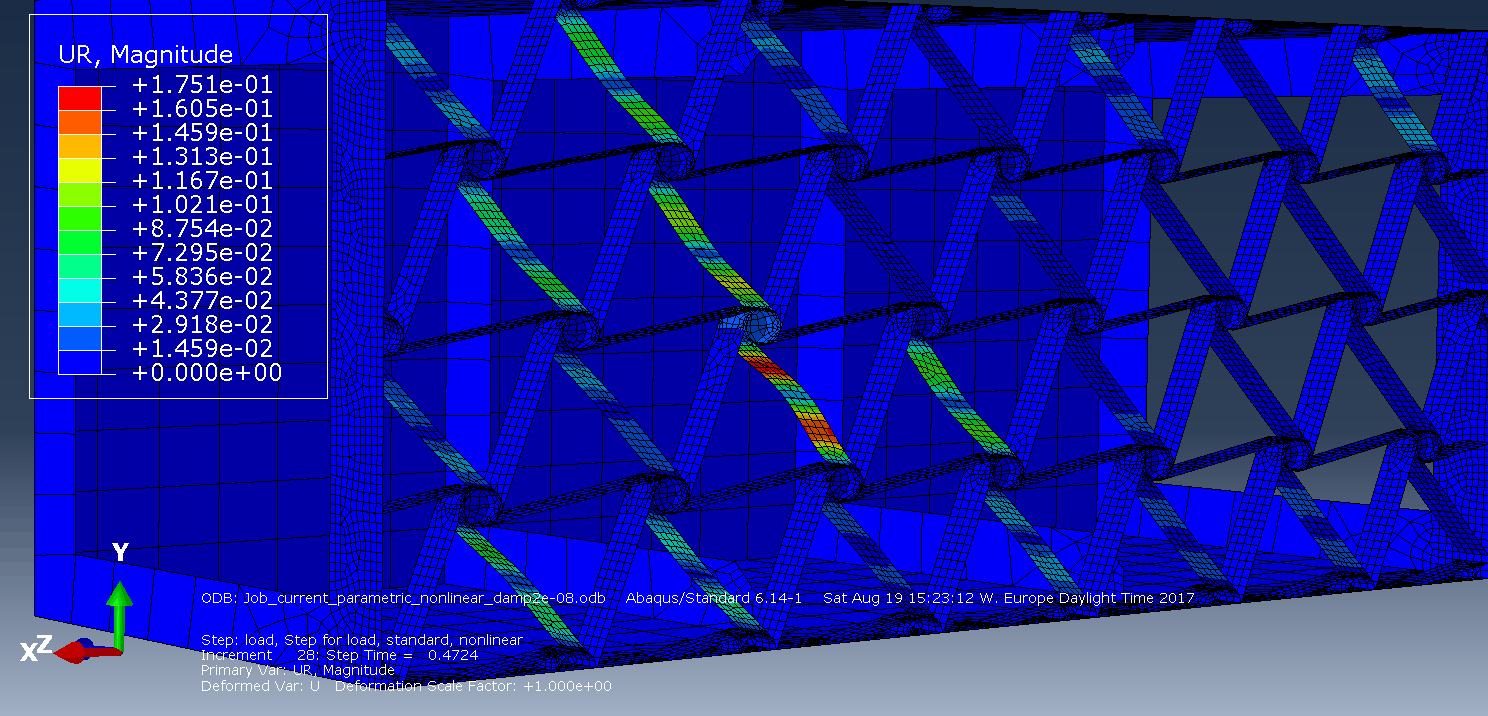
\includegraphics[width=0.8 \textwidth]{figures/result-sim/1-UR}
    \caption[Baseline model response when the fraction of load applied equals to 47\% of the prescribed load (700 N)]{Baseline model response when the fraction of load applied equals to 47\% of the prescribed load (700 N). Buckling has appeared at the tip of the wing-box due as an initial response to the load that it is being introduced.}\label{fig:1-UR}
  \end{figure}

  This is the point at which the local instabilities are such that there is need of adding artificial damping factor in order to capture the structure dynamics. After this point, artificial damping is essential for the simulation to continue. As it was explained in Subsection \ref{subsec:nonlinear_results_model}, special care needs to be taken to ensure that the inclusion of artificial damping factor is not leading to inaccurate results due to over-damping of the structure. This can be done by comparing the fraction of the static energy that it is dissipated with to the external work that is introduced into the system. The Figure \ref{fig:energy} makes this comparison possible. It can be seen that effectively, the energy statically dissipated through automatic stabilization is negligible in comparison with the external work. This figure also shows the abrupt increment in external work at the point where the structure collapses due to sudden buckling of the chiral ligaments.

  \begin{figure}[!htpb] %Energy plot
    \centering
    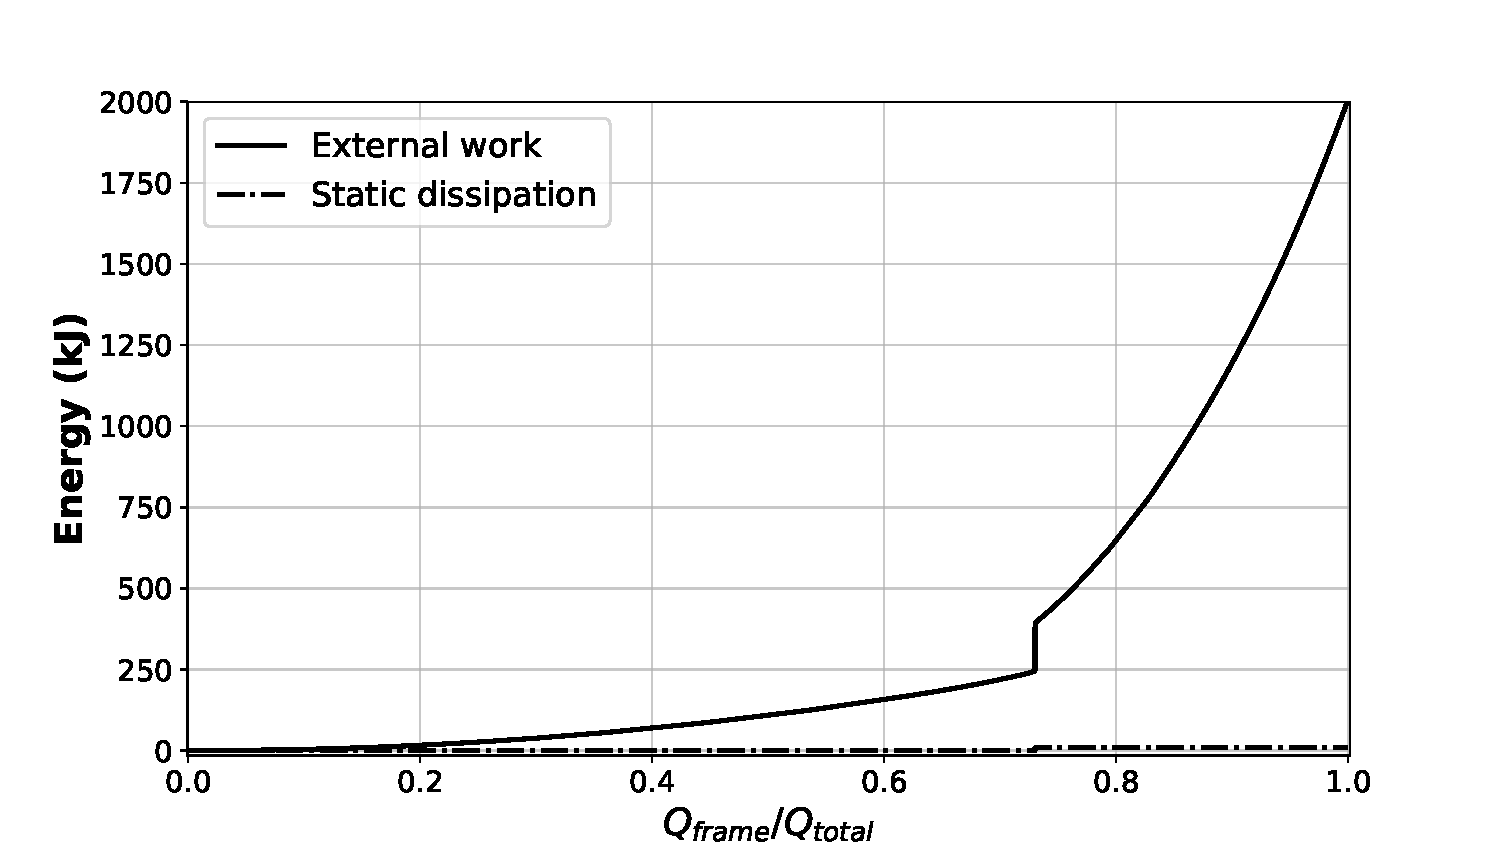
\includegraphics[width=0.8 \textwidth]{figures/result-sim/energy}
    \caption[External work and static dissipation for a simulation of the baseline configuration]{External work and static dissipation for a simulation of the baseline configuration. It can be seen that the static dissipation through automatic stabilization is negligible in comparison with the external work showing that the inclusion of artificial damping factor is unluckily to be leading to inaccurate results. The abrupt change in the external work shows the point where structure collapses due to sudden buckling of the chiral ligaments.}\label{fig:energy}
  \end{figure}

  In order to see the overall system response as load increases, a displacement-force curve can be plotted. The Figure \ref{fig:forceDisplacement-far} shows the wing-box twist adaptation as load increases. In this plot, results from the nonlinear simulations are shown as the set of scatter points while the dotted line represents the forecast response by the linear simulation. In the case shown, the linear simulation arises a value for the twist at the wing-box tip $\phi_{\mathrm{tip}}$ equal to $-0.196$ degrees while the nonlinear simulation predicts a final twist of $-1.248$ degrees. This shows that the problem under study is highly nonlinear.

  \begin{figure}[!htpb] %ForceDisplacement-far
    \centering
    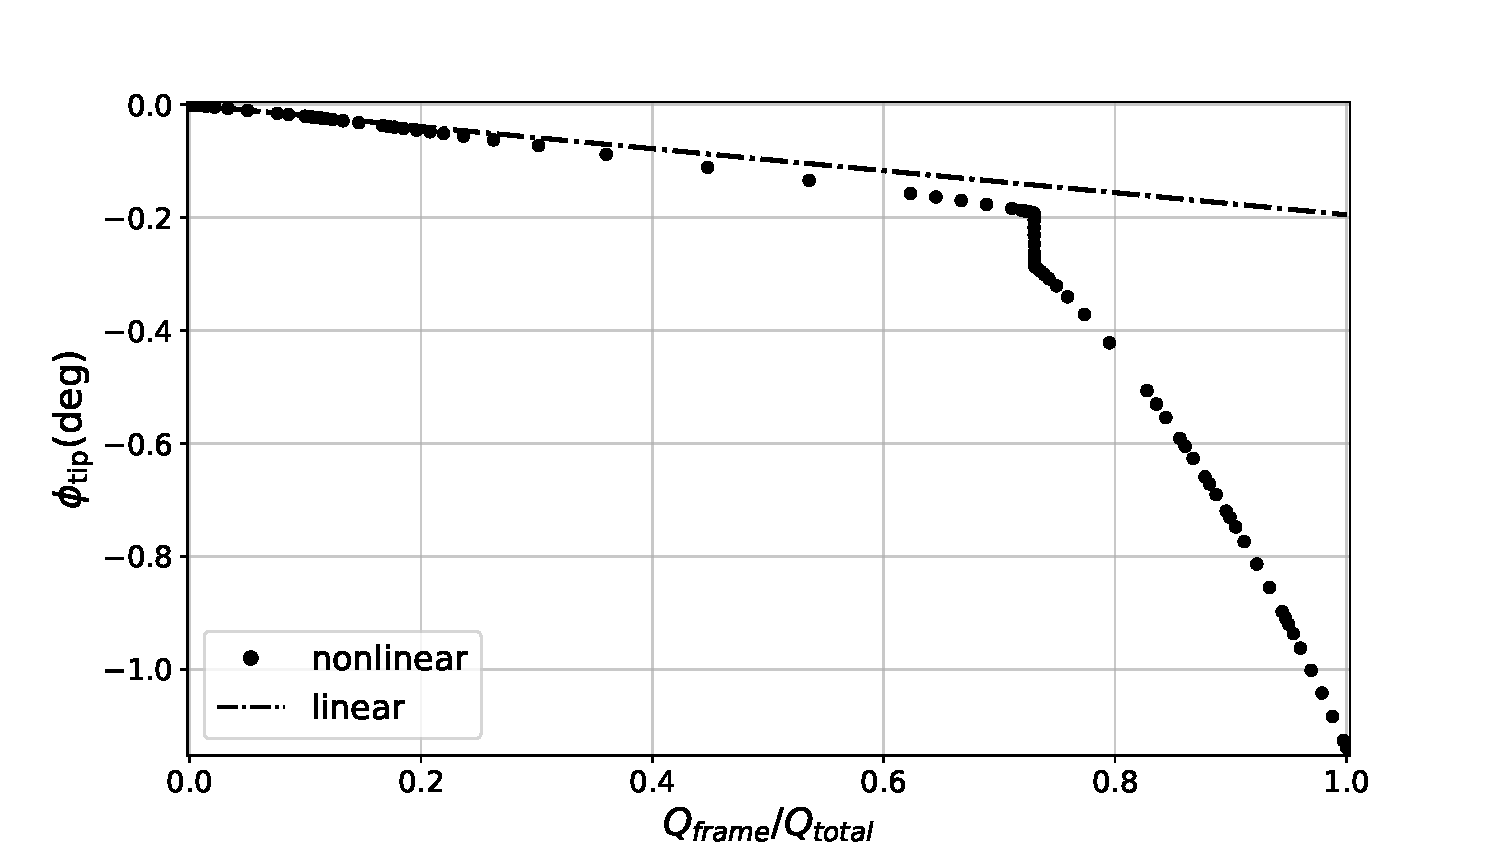
\includegraphics[width=0.8 \textwidth]{figures/result-sim/forceDisplacement-far}
    \caption[Displacement-force curve for the baseline configuration]{Displacement-force curve for the baseline configuration. Two breakdowns for the buckling deformation are shown in the plot. The first one is located at the point where the fraction of applied load equals to $73\%$ and the second one at the point where the fraction is $96\%$.}\label{fig:forceDisplacement-far}
  \end{figure}

  The nonlinear response also shows the point where the structure collapses, when $73\%$ of the prescribed load has been applied. The colour contour plot of the total rotational displacement over the solution model is shown in Figure \ref{fig:2-UR}. This figure shows severe buckling occurring at the root of the lattice chiral structure.

  \begin{figure}[!htpb] %Second step in the deformation
    \centering
    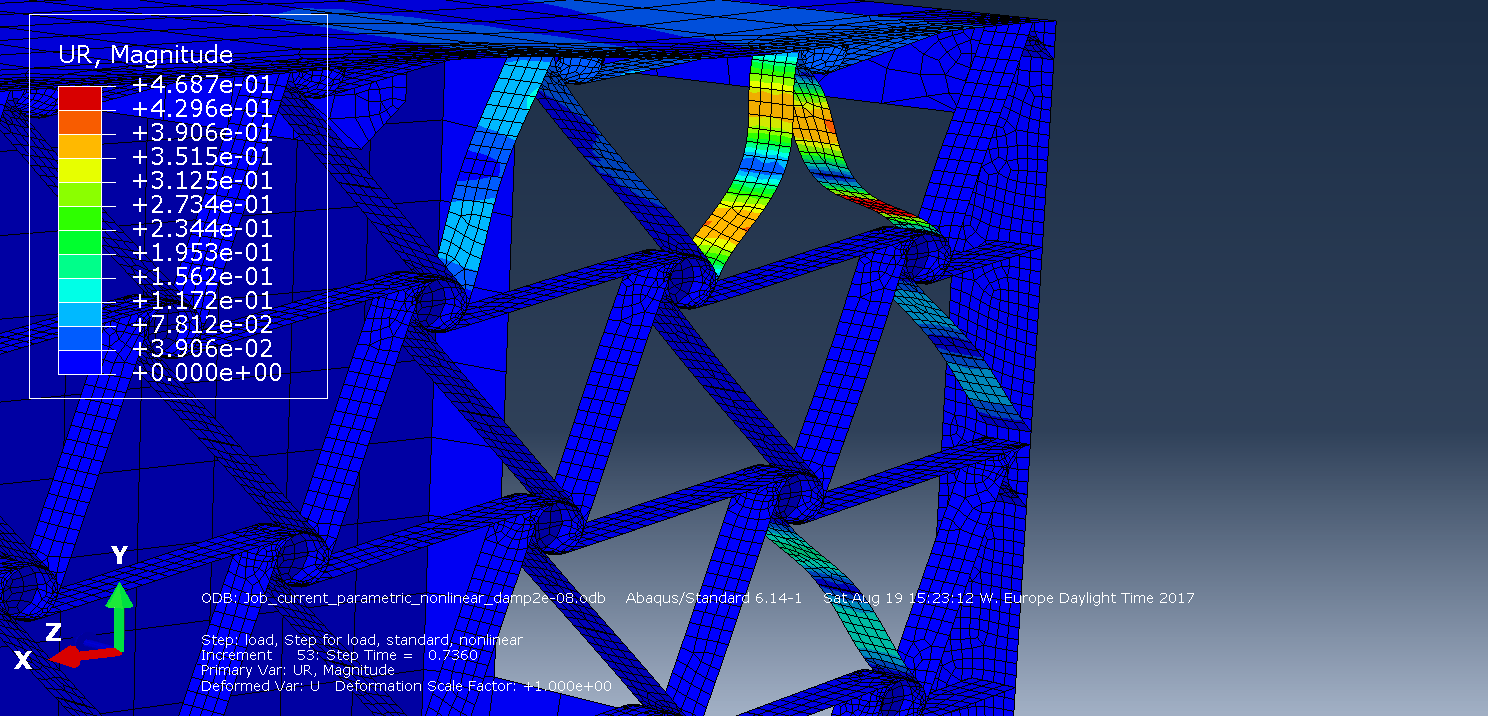
\includegraphics[width=0.8 \textwidth]{figures/result-sim/2-UR}
    \caption[Baseline model response when the fraction of load applied equals to 73\% of the prescribed load (700 N)]{Baseline model response when the fraction of load applied equals to 73\% of the prescribed load (700 N). Severe buckling deformation appears in those chiral ligaments located at the root and with a higher $y$ coordinate. This is the point when the structure collapses and the twist increases for small increments in load.}\label{fig:2-UR}
  \end{figure}

  In a further stage of the simulation, the structure enters the post-buckling regime and the instabilities propagate to other parts of the lattice chiral structure, as it can be seen in Figure \ref{fig:3-UR}. Here it can be seen that the instabilities are more generalized and buckling appears in more ligaments apart from those at the root. Under certain conditions, this generalized state can produce a second sudden variation in the slope of the displacement-force curve, showing a third effective stiffness. 

  \begin{figure}[!htpb] %Third step in the deformation
    \centering
    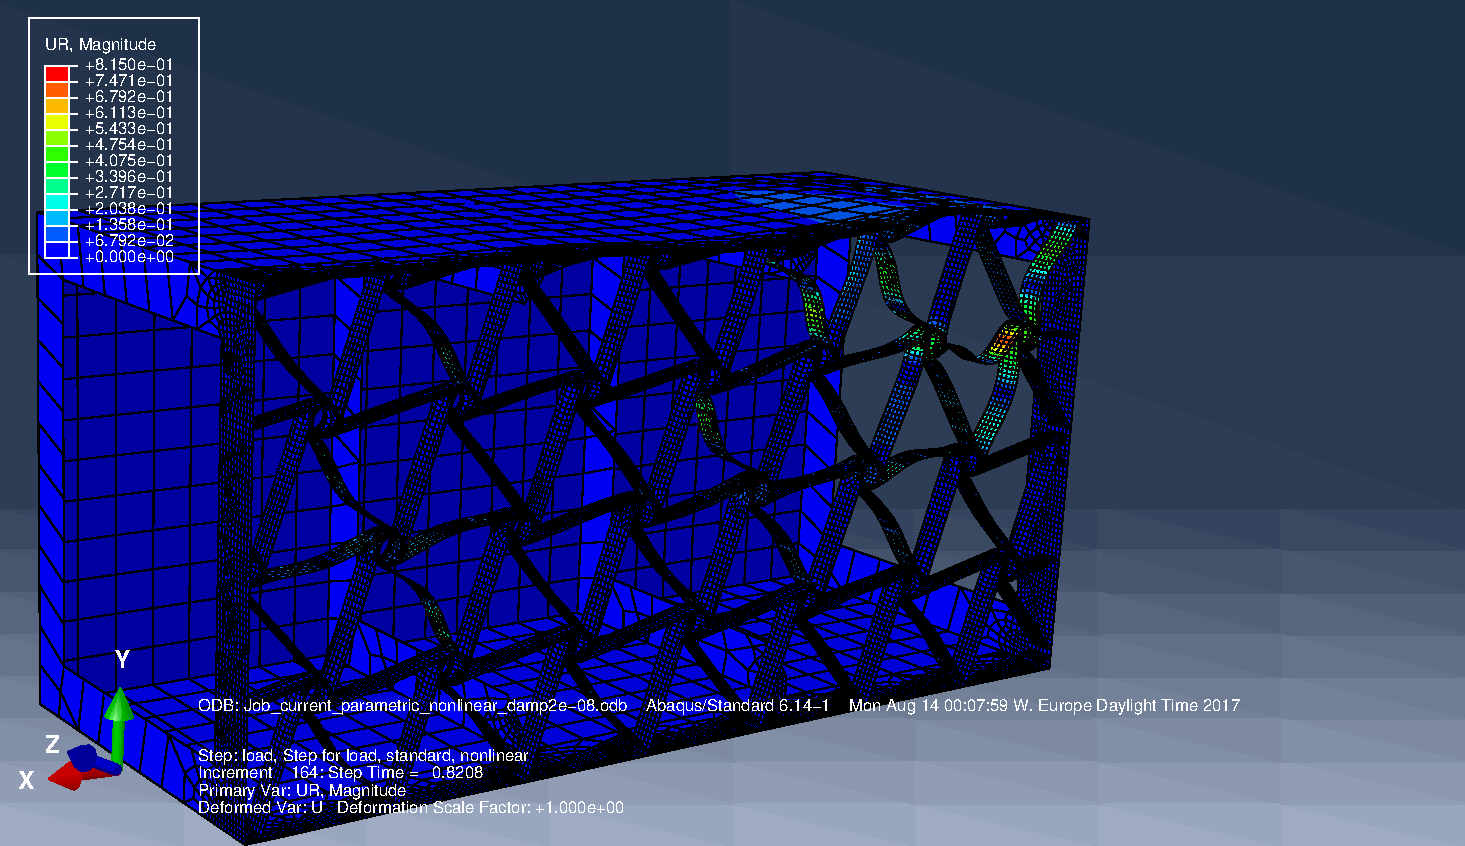
\includegraphics[width=0.8 \textwidth]{figures/result-sim/3-UR}
    \caption[Baseline model response when the fraction of load applied equals to 96\% of the prescribed load (700 N)]{Baseline model response when the fraction of load applied equals to 96\% of the prescribed load (700 N). In this case, not only the ligaments located at the root show severe buckling but also, other located at different points of the chiral lattice has started to buckle at the same time, inducing rapidly growing deformation for small increments in load.}\label{fig:3-UR}
  \end{figure}

\clearpage
\section{Parametric study on the computational model} \label{sec:computationalParametricStudy_results_sim}
  %
  % *Cbox-t: Minimum seems to be 0.8. For less values, the simulation crashes.
  The aim of this section is to show the effect of each parameter on the nonlinear response of the structure. The parameters  included in the analysis are the following:
  %
  \begin{itemize}
    \item Wing-box thickness \boxt
    \item Number of unit cells in the transversal direction $M$
    \item Number of unit cells in the spanwise direction $N$
    \item Chiral node depth \chiB
    \item Chiral node radius \chir
    \item Chiral lattice thickness \chit
    \item Chiral ligament half length \chiL
    \item Dimensionless ligament eccentricity \chie
  \end{itemize}

  \subsection{Wing-box thickness} \label{subsec:Cbox_t_para}
    %Summary of results
    %   - Range: 0.8, 1, 1.2, 1.4
    %   - This parameters has high influence in the appearance of buckling or not
    %   - Force displacement plot
    %       - For the one close. It is possible to see that for all the cases except one, the response is linear at the beggining, but non-linearities become relevant when the applied load is \%20 approximatelly. Therefore, this offset between the linear and nonlinear is constant for \ref{fig:result-sim/cbox/force_displacement-close}
    %   - For 1.4
    %       - No buckling at the root
    %       - Buckling appears first at the first ligaments after the inner rib located in higer x position
    %       - \ref{fig:result-sim/cbox/1coma4-800N}
    %       - A simular behaviour is shown for the linear simulation. There is for this case, small difference between computing the linear and the nonlinear simulations
    %       - \ref{fig:result-sim/cbox/1coma4-800N-linear}
    %   - For 1.2
    %       - Similar result
    %   - For 1.0
    %       - Similar, result but now it can be seen how there are some lattices that are buckling as well close to the root
    %   - For 0.8
    %       - For this case, the Figure \ref{fig:result-sim/cbox/force_displacement-close} shows that there is an abrupt collapse of the structure when \%60 of the load has been applied.
    %       - Show \ref{fig:result-sim/cbox/0coma8-800N-1}
    %       - The structure collapses a this point, inducing considerable local deformation at the point where the ligaments present a more severa buckling, at the root.
    %       - The figure \ref{fig:result-sim/cbox/force_displacement-far} shows the evolution of the twist for this case, in the post-buckling region until all the load has been applied. In this region, each of the lattice that buckled increase its deformation. There aren't any new lattices that buckle
    %       - Another remark to make is that the linear simulation was unable to capture all the dynamics ocurring for this case.
    %
    %    -Table summary: In Table \ref{tab:ur1_cbox_t} the value of the twist from each of the cases considered. It shows the maximum twist achieved for each of the cases together with a reference to the maximum desviation from the mean twist for each of the twist values that are obtained from different sources.
    %       - In Table \ref{tab:ur1_cbox_t}, the maximum mesh node vertical displacement $v$ on the upper skin of the wing box is shown. For the case $t_{\mathrm{box}} = 0.8$mm, the point where the maximum vertical displacement is shown close to the root, where $x_{v_{\mathrm{min}}}} = 0.334$. OK

    In the present subsection the effect of different values for the wing-box thickness \boxt on the structure response is investigated. The geometric representation of the wing-box thickness \boxt can be seen in Figure \ref{fig:wing-box-internalParameters}.

    The results from the simulations carried out can be seen in Table \ref{tab:para_cbox}. In the table, the twist at the tip of the wing-box for the Abaqus nonlinear simulation $\phi_{\mathrm{tip}}$ and for the linear simulation $\tilde{\phi}_{\mathrm{tip}}$ are shown. This result is obtained by evaluating the value of the angular deformation $u$ at a number of mesh elements located in different parts of the wing-box tip rib, as explained in the Subsection \ref{subsec:postProc_computationalModel}. Therefore, the maximum deviation between the individual values and the calculated mean twist has also been included. Finally, the Table \ref{tab:para_cbox} shows the maximum vertical displacement found in the nodes located in the upper wing-box skin.

    \begin{table}[!htpb] %Table results cbox_t
      \centering
      \begin{tabular}{|l|l|l|l|l|l|l|l|l|}
      \hline
      \boxt (mm)& $\phi_{\mathrm{tip}}$ (deg) & $e(\phi_{\mathrm{tip}}) (\%)$ & $\tilde{\phi}_{\mathrm{tip}}$ (deg) & $e(\tilde{\phi}_{\mathrm{tip}}) (\%)$ & $v_{\mathrm{max}}$ & $\hat{z}_{v_{\mathrm{max}}}$ & $\hat{x}_{v_{\mathrm{max}}}$ \\ \hline
      0.6 & -14.331 & 11.13  & -0.27  & -14.259 & 0.121 & -85.506 & 1 & 0.971 \\ \hline
      0.8 & -1.934  & 11.43  & -0.223 & -15.178 & 0.546 & -15.915 & 1 & 0.334 \\ \hline
      1   & -0.403  & 14.651 & -0.2   & -19.923 & 0.546 & -4.741  & 1 & 0.334 \\ \hline
      1.2 & -0.221  & 15.031 & -0.178 & -21.074 & 0.121 & -1.246  & 1 & 0.971 \\ \hline
      \end{tabular}
      \caption[Results from the parametric study on the wing-box thickness]{Results from the parametric study on the wing-box thickness \boxt. The results show the mean twist at the tip of the wing-box for the Abaqus nonlinear simulation $\phi_{\mathrm{tip}}$ and for the linear simulation $\tilde{\phi}_{\mathrm{tip}}$. The maximum relative error of the mean calculation, expressed as percentage, for these two magnitudes is $e(\phi_{\mathrm{tip}})$ and $e(\tilde{\phi}_{\mathrm{tip}})$, respectively. The table also shows the maximum vertical displacement $v_{\mathrm{max}}$ among all the mesh nodes located on the upper skin of the wing-box and the dimensionless position in the spanwise direction $\hat{x}_{v_{\mathrm{max}}}$ and in the chordwise direction $\hat{z}_{v_{\mathrm{max}}}$ of the node that shows $v = v_{\mathrm{max}}$.}
      \label{tab:para_cbox}
    \end{table}

    The displacement-force curve for each of the values of \boxt studied can be seen in Figure \ref{fig:forceDisplacement-far-Cbox_t}. It can be seen that the structure collapses for the cases of \boxt$= 0.6$ mm, \boxt$= 0.8$ mm and \boxt$= 1.0$ mm, when the load applied reaches 40\%, 64\% and 97\% of the total prescribed load, respectively. This result already shows the relevance of the wing-box thickness \boxt in the triggering of the collapsing buckling. A detailed view of the nonlinear response of the structure for the different analysed cases is shown in Figure \ref{fig:forceDisplacement-close-Cbox_t}. Here, the difference between the linear and the nonlinear is represented and it can be seen that the gap between the two responses increases as the value of \boxt decreases. In the Table \ref{tab:para_cbox}, comparing the values of $\phi_{\mathrm{tip}}$ and $\tilde{\phi}_{\mathrm{tip}}$ provides information of the huge difference in the final value of the twist between the nonlinear and the linear response when the buckling occurs and it is captured in the simulation. For example, for \boxt$= 0.8$ mm, the value of the tip twist from the linear simulation $\tilde{\phi}_{\mathrm{tip}}$ is 12\% of the value estimated from the nonlinear simulation \phinonlin.

    \begin{figure}[!htpb] %force_displacement-far
      \centering
      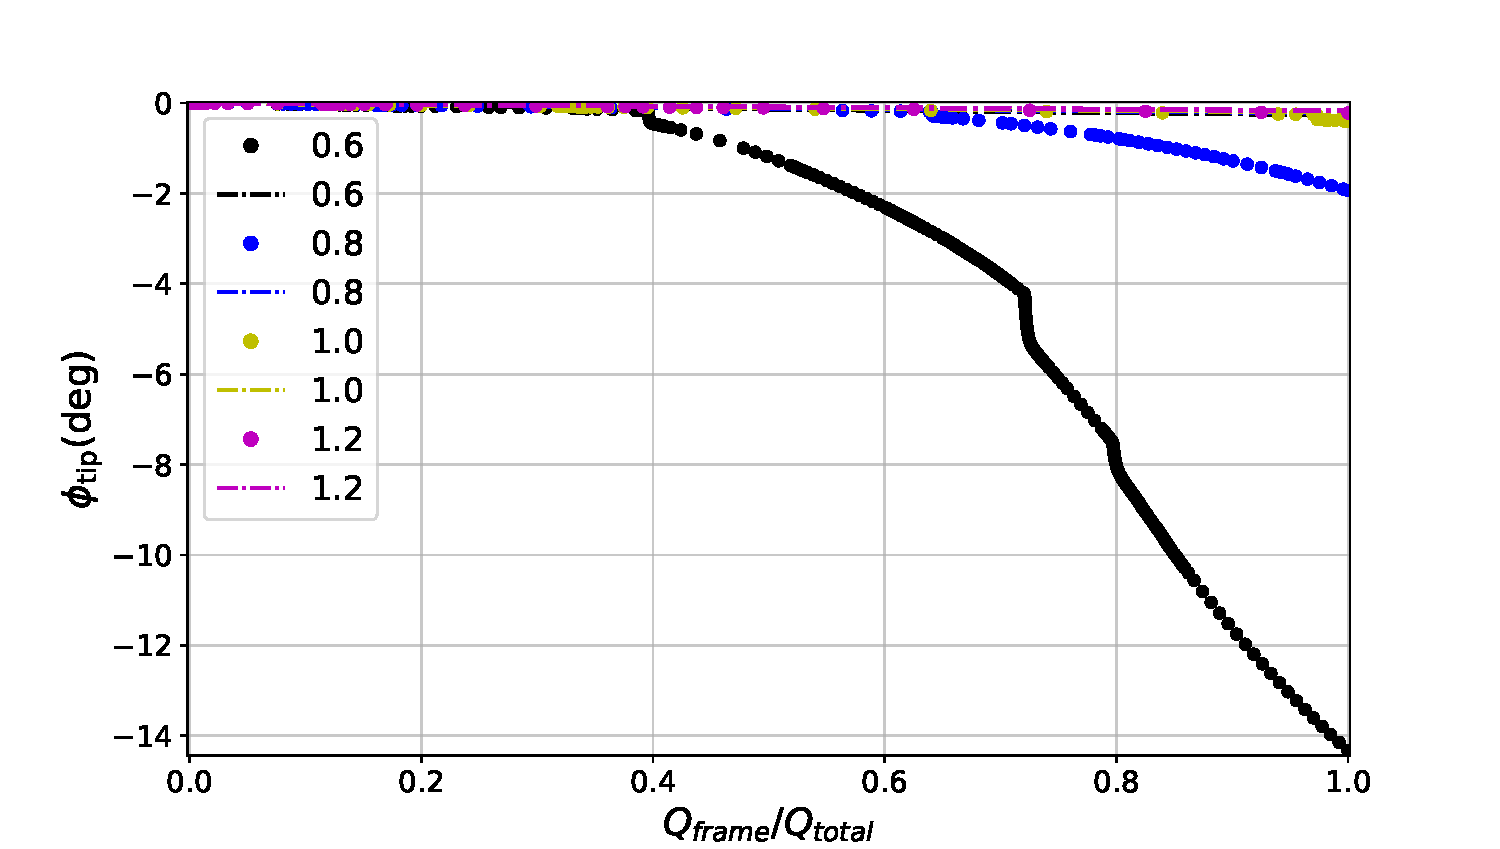
\includegraphics[width=0.8 \textwidth]{figures/result-sim/cbox/force_displacement-far}
      \caption[Displacement-force curve for various values of the wing-box thickness]{Displacement-force curve for various values of the wing-box thickness \boxt. For all the cases shown, the force applied was located on the upper flange of the tip rib and its magnitude was equal to -800 N.}\label{fig:forceDisplacement-far-Cbox_t}
    \end{figure}

    \begin{figure}[!htpb] %force_displacement-close
      \centering
      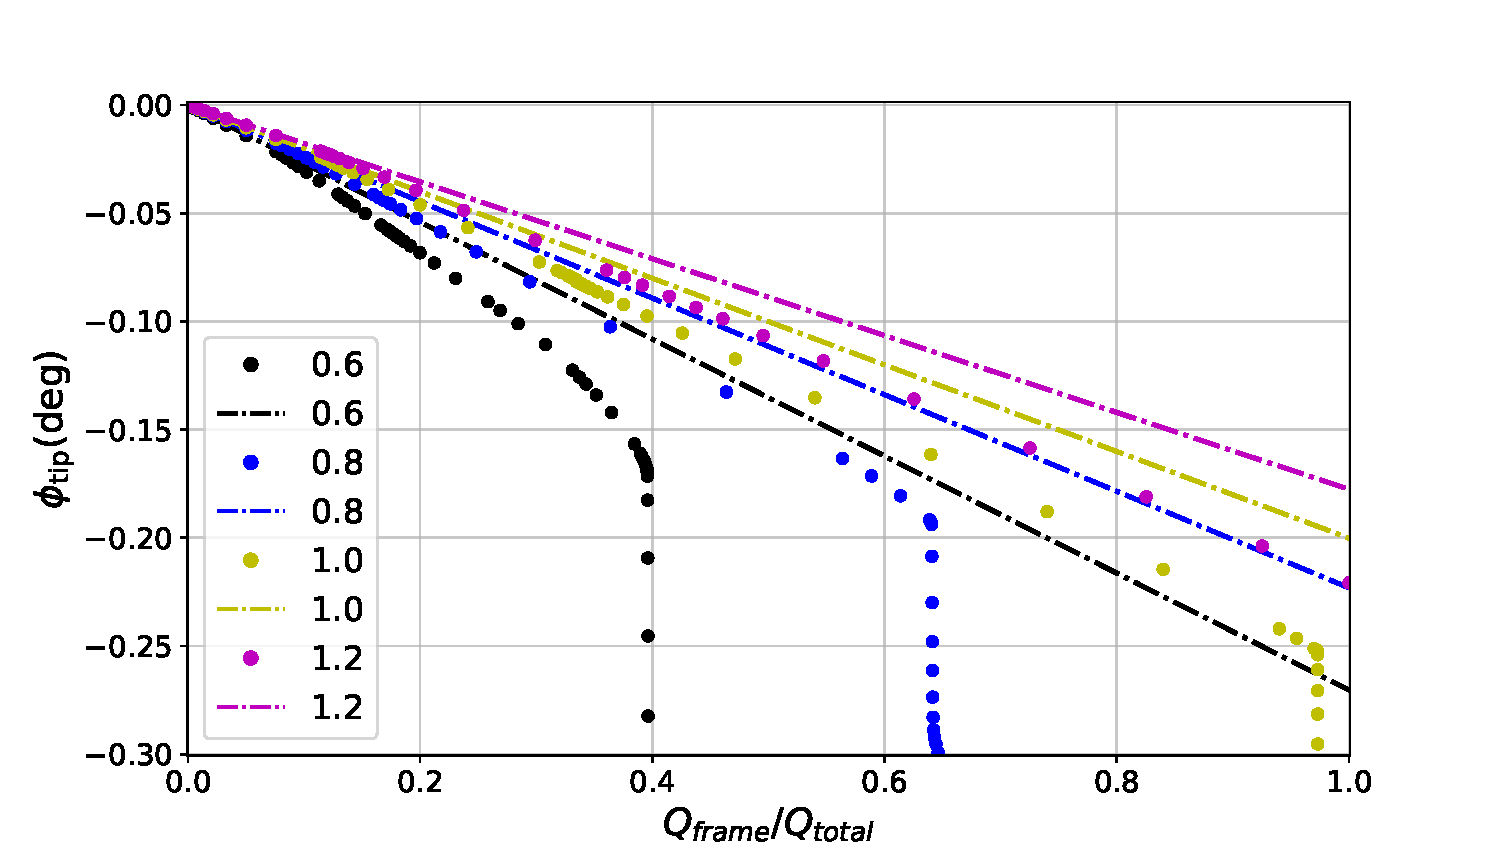
\includegraphics[width=0.8 \textwidth]{figures/result-sim/cbox/force_displacement-close}
      \caption[Detail of the displacement-force curve for various values of the wing-box thickness]{Detail of the displacement-force curve for various values of the wing-box thickness \boxt. For all the cases shown, the force applied was located on the upper flange of the tip rib and its magnitude was equal to -800 N.}\label{fig:forceDisplacement-close-Cbox_t}
    \end{figure}

    The differences in response for the different cases are also visually evaluated using colour contour plots of total rotational displacement. Such a visualization is shown in Figure \ref{fig:1coma2-800N-cbox_t} for the case of wing-box thickness \boxt$= 1.2$. It can be seen that buckling does not propagate to other parts of the lattice and it stays where it had appeared on first place, at the first ligaments after the inner rib located further from the root. In this case, the value of wing-box thickness \boxt$= 1.2$ mm makes the structure sufficiently stiff in bending and therefore, buckling does not appear at the root causing the structure collapse.

    \begin{figure}[!htpb] %UR
      \centering
      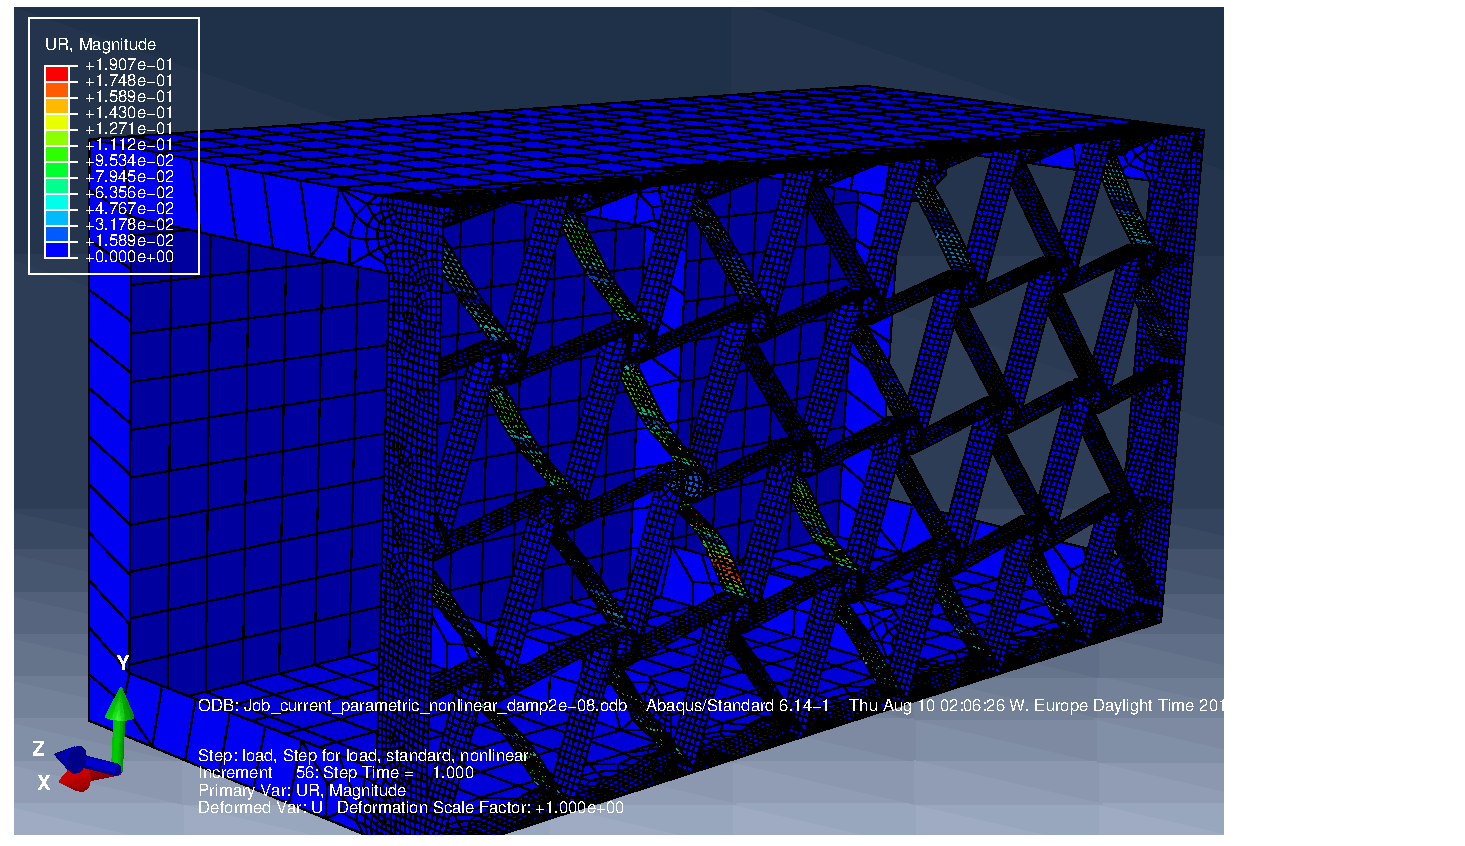
\includegraphics[width=0.8 \textwidth]{figures/result-sim/cbox/1coma4-800N}
      \caption[Color contour representation of the total angular displacement of the mesh elements on the deformed structure for \boxt$ = 1.2$ mm]{Color contour representation of the total angular displacement of the mesh elements on the deformed structure for \boxt$ = 1.2$ mm. This case is shown after all the prescribed load (800 N) has been applied. The elastic instabilities had appeared at the wing tip and they have not propagated to the rot causing the structure collapse.}\label{fig:1coma2-800N-cbox_t}
    \end{figure}

    On the other hand, in Figure \ref{fig:0coma8-800N-cbox_t} the same plot is shown for a value of wing-box thickness \boxt$= 0.8$ mm, after all the prescribed load (800 N) has been applied. This figure shows how severe deformation due to buckling is occurring in the ligaments at the root. It is possible to see that some local deformation has been induced into the upper skin of the wing-box in between the root and the first inner rib. As shown in Table \ref{tab:para_cbox}, for the case $t_{\mathrm{box}} = 0.8$ mm, the point with maximum displacement $v$ in the $y$ direction is shown to appear close to the root, where $\hat{x}_{v_{\mathrm{max}}} = 0.334$.

    \begin{figure}[!htpb] %UR
      \centering
      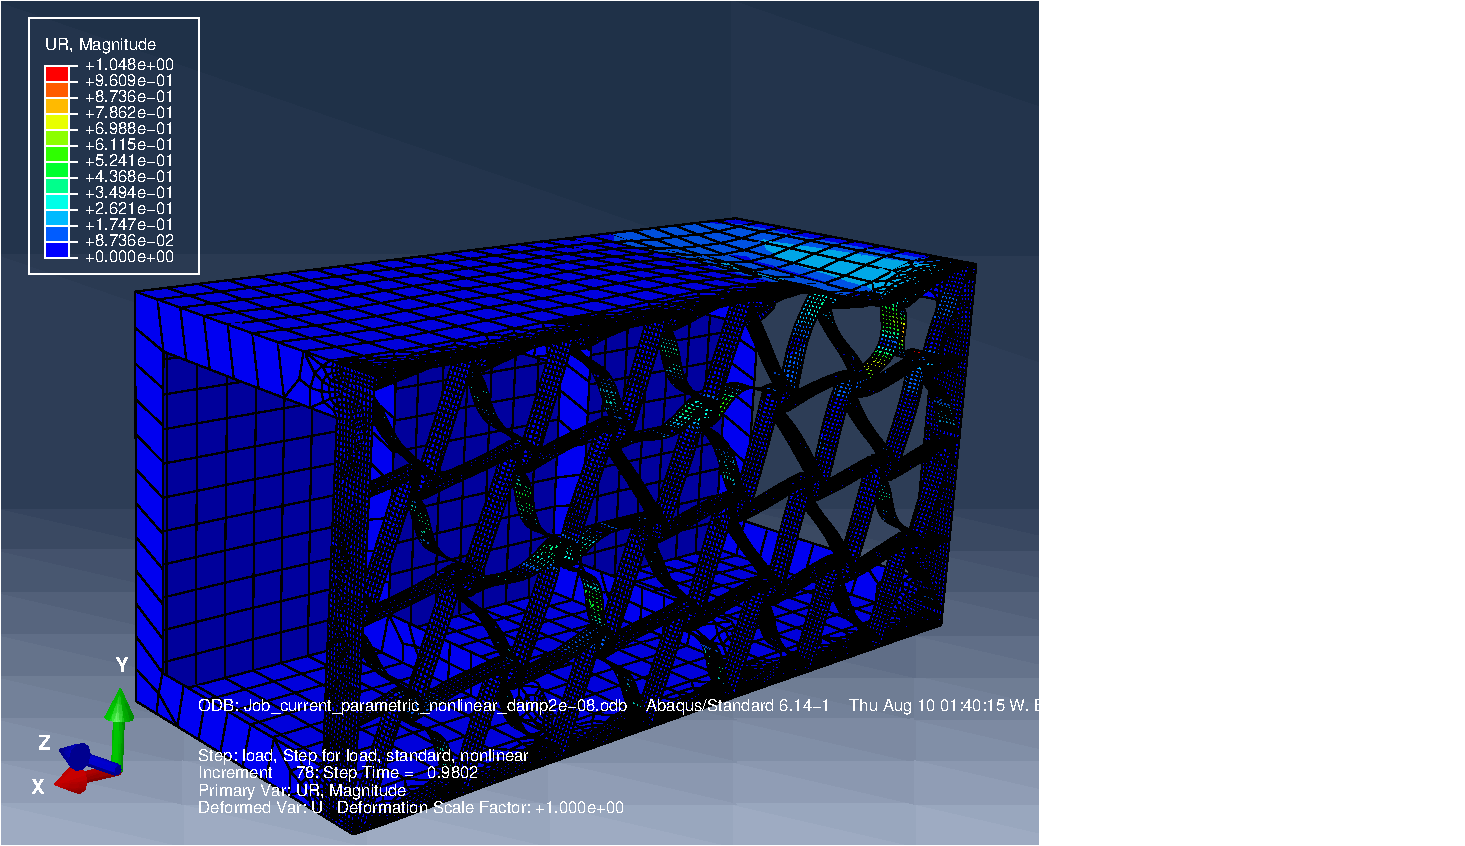
\includegraphics[width=0.8 \textwidth]{figures/result-sim/cbox/0coma8-800N-2}
      \caption[Color contour representation of the total angular displacement of the mesh elements on the deformed structure for \boxt$ = 0.8$ mm]{Color contour representation of the total angular displacement of the mesh elements on the deformed structure for \boxt$ = 0.8$ mm. This case is shown after all the prescribed load (800 N) has been applied. The appearance of elastic instabilities at the ligaments at the root has induced the structure collapse and local deformation on the wing-box skin.}\label{fig:0coma8-800N-cbox_t}
    \end{figure}

    Finally, for the case of \boxt$= 0.6$ mm, it can be seen that the collapse of the structure occurs when just 40\% of the prescribed load has been applied. For this case, Figure \ref{fig:forceDisplacement-far-Cbox_t} shows a second change in the slope of the force-displacement curve when approximately 72\% of the prescribed load has been applied. This second stage of the collapse of the structure appears when the elastic instabilities propagate from the ligaments at the root to other ligaments located closer to the tip of the structure. In Figure \ref{fig:0coma6-800N-cbox_t}, this generalized buckling can be seen at the moment when the second change in the slope of the force-deformation curve occurs. All those ligaments that have just started to deform, causing the wing-box sudden adaptation in twist for the second time. 

    \begin{figure}[!htpb] %UR
      \centering
      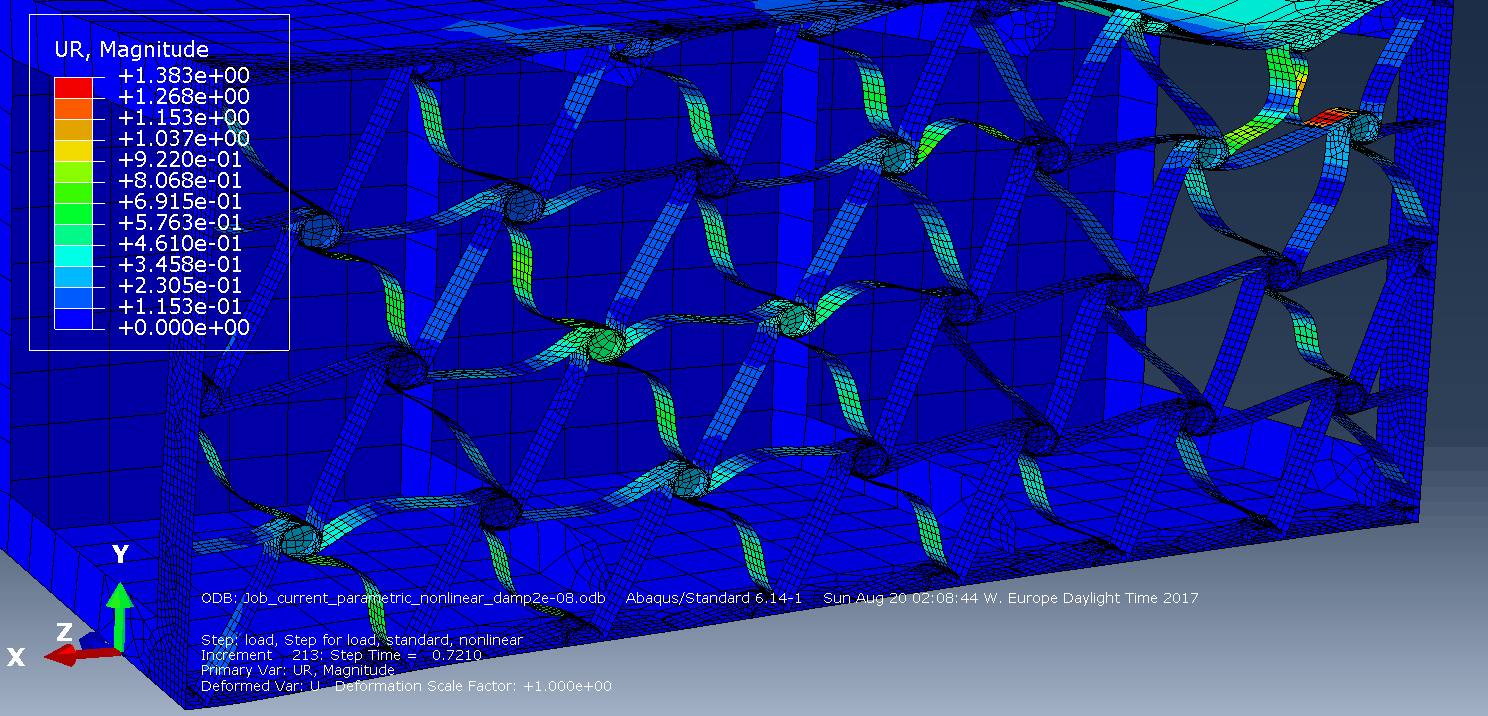
\includegraphics[width=0.8 \textwidth]{figures/result-sim/cbox/0coma6-800N-2}
      \caption[Color contour representation of the total angular displacement of the mesh elements on the deformed structure for \boxt$ = 0.6$ mm]{Color contour representation of the total angular displacement of the mesh elements on the deformed structure for \boxt$ = 0.6$ mm. This case is shown when 72\% of the prescribed load (800 N) has been applied. The figure shows how the elastic instabilities have extended to the majority of the ligaments in the chiral lattice.}\label{fig:0coma6-800N-cbox_t}
    \end{figure}

    A further study is performed in order to see the relationship between the wing-box thickness and the value of the force applied that induces the structure collapse. As a result, the plot shown in Figure \ref{fig:force_cbox_t} is produced. It can be seen that relatively small variations in \boxt produce considerable increments in the load required to trigger the buckling-induced twist adaptation of the wing-box, as it has been already mentioned. For example, for \boxt$ = 0.6$ mm, the magnitude of the force required to activate the mechanism is 300 N, while for \boxt$ = 0.8$ mm, the magnitude raises up to 525 N.

    \begin{figure}[!htpb] %force_plot
      \centering
      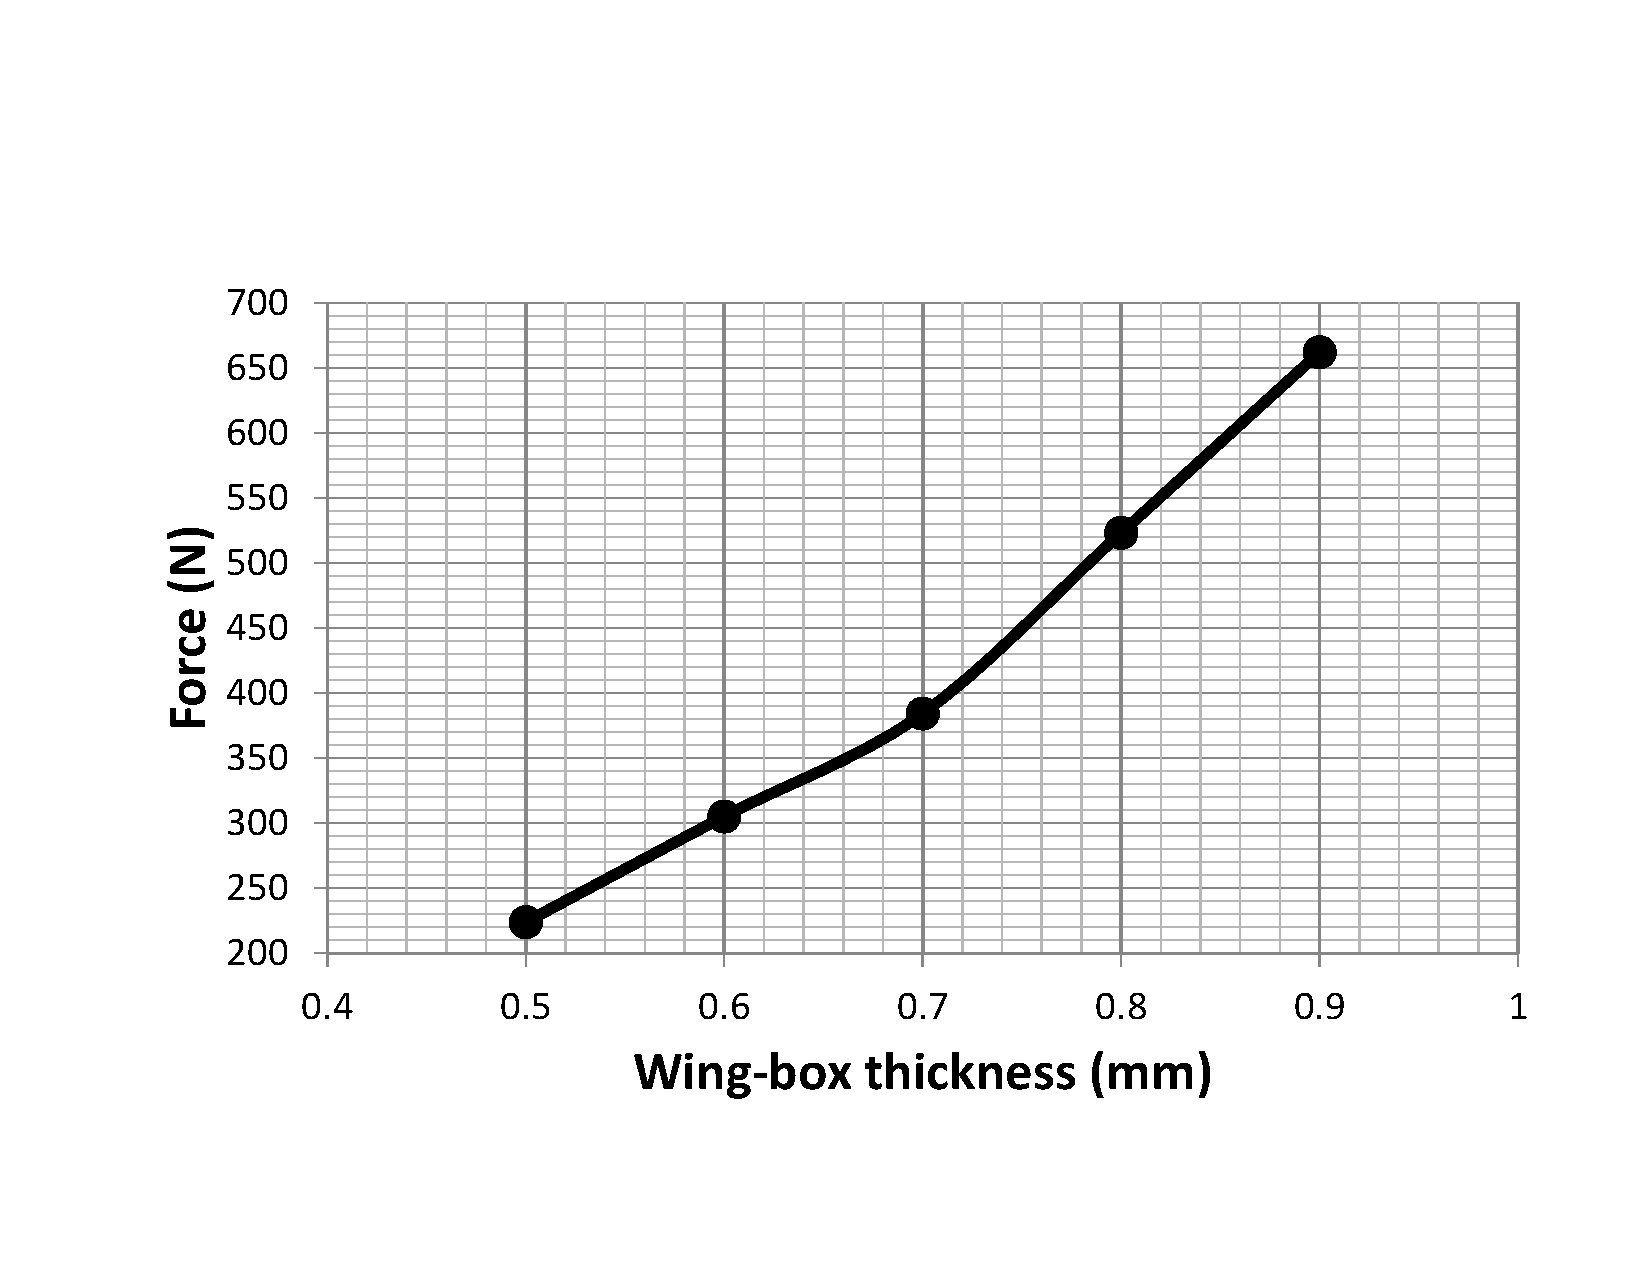
\includegraphics[width=0.8 \textwidth]{figures/result-sim/cbox/force_cbox_t}
      \caption[Force that induces the structure to collapse as a function of the wing-box thickness]{Force that induces the structure to collapse as a function of the wing-box thickness \boxt.}\label{fig:force_cbox_t}
    \end{figure}

  \clearpage
  \subsection{Number of unit cells in the chiral lattice} \label{subsec:MandN_para}
    %
    %   -> For M:
    %       -It was neccessary to increase the load up to 1200N to see the wing-box with $M = 4$ to collapse

    Now the effect of the number of units cells in the transversal direction $M$ and in the spanwise direction $N$ on the structural response is investigated. These two parameters are responsible of the height and the length of the wing-box, respectively. The division of the chiral lattice in $M$ units cells in the transversal direction and in $N$ units cells in the spanwise direction can be seen in Figure \ref{fig:lattice-NandM}.

    Firstly, the number of unit cells in the transversal direction $M$ is varied. This parameter modifies the height of the model. Similarly as it was done for the study of the wing-box thickness \boxt influence in the structure response, the results from the different simulations are shown in Table \ref{tab:para_M}. Also, the displacement-force curve is shown in Figure \ref{fig:forceDisplacement-far-M}. It can be seen from the results that increasing $M$ results in a decrement of the structure sensitivity to buckling. In order to be able to onset the elastic instabilities for $M > 3$, the simulations are executed for a prescribed load of 1200 N.

    \begin{table}[!htpb] %Results of M
      \centering
      \begin{tabular}{|l|l|l|l|l|l|l|l|l|}
      \hline
      $M$ & $\phi_{\mathrm{tip}}$ (deg) & $e(\phi_{\mathrm{tip}}) (\%)$ & $\tilde{\phi}_{\mathrm{tip}}$ (deg) & $e(\tilde{\phi}_{\mathrm{tip}}) (\%)$ & $v_{\mathrm{max}}$ & $\hat{z}_{v_{\mathrm{max}}}$ & $\hat{x}_{v_{\mathrm{max}}}$ \\ \hline
      3 & -9.672 & 11.43 & -0.335 & -15.177 & -55.962 & 1   & 0.971 \\ \hline
      4 & -1.221 & 18.13 & -0.289 & -24.409 & -11.467 & 1   & 0.546 \\ \hline
      5 & -0.385 & 15.3  & -0.267 & -21.211 & -1.747  & 0.9 & 0.971 \\ \hline
      \end{tabular}
      \caption[Results from the parametric study on the number of unit cells in the transversal direction]{Results from the parametric study on the number of unit cells in the transversal direction $M$. The results show the mean twist at the tip of the wing-box for the Abaqus nonlinear simulation $\phi_{\mathrm{tip}}$ and for the linear simulation $\tilde{\phi}_{\mathrm{tip}}$. The maximum relative error of the mean calculation, expressed as percentage, for these two magnitudes is $e(\phi_{\mathrm{tip}})$ and $e(\tilde{\phi}_{\mathrm{tip}})$, respectively. The table also shows the maximum vertical displacement $v_{\mathrm{max}}$ among all the mesh nodes located on the upper skin of the wing-box and the dimensionless position in the spanwise direction $\hat{x}_{v_{\mathrm{max}}}$ and in the chordwise direction $\hat{z}_{v_{\mathrm{max}}}$ of the node that shows $v = v_{\mathrm{max}}$.}
      \label{tab:para_M}
    \end{table}

    From the results shown in Table \ref{tab:para_B} it can be seen how for the case of $M = 3$, the point that shows $v = v_{\mathrm{max}}$ is located at the wing-box tip where $\hat{x}_{v_{\mathrm{max}}} = 0.971$, due to the high twist of the structure. However, for $M = 4$, the location of the point with $v = v_{\mathrm{max}}$ is at $\hat{x}_{v_{\mathrm{max}}} = 0.546$ showing the point at which local deformation occurs. The value of the twist at the tip \phinonlin has been reduced in 12\% of what it was for $M = 3$. This shows that the structure increases its shear stiffness as the height of the wing-box increases. For $M = 5$, the structure is sufficiently stiff that $v_{\mathrm{max}}$ appears approximately at the point where the load is applied and the collapse of the structure does not occur. This shows that deformation is only achieved in the vicinity of the load introduction point due to the high stiffness in shear of the structure.

    \begin{figure}[!htpb] %force_displacement-far
      \centering
      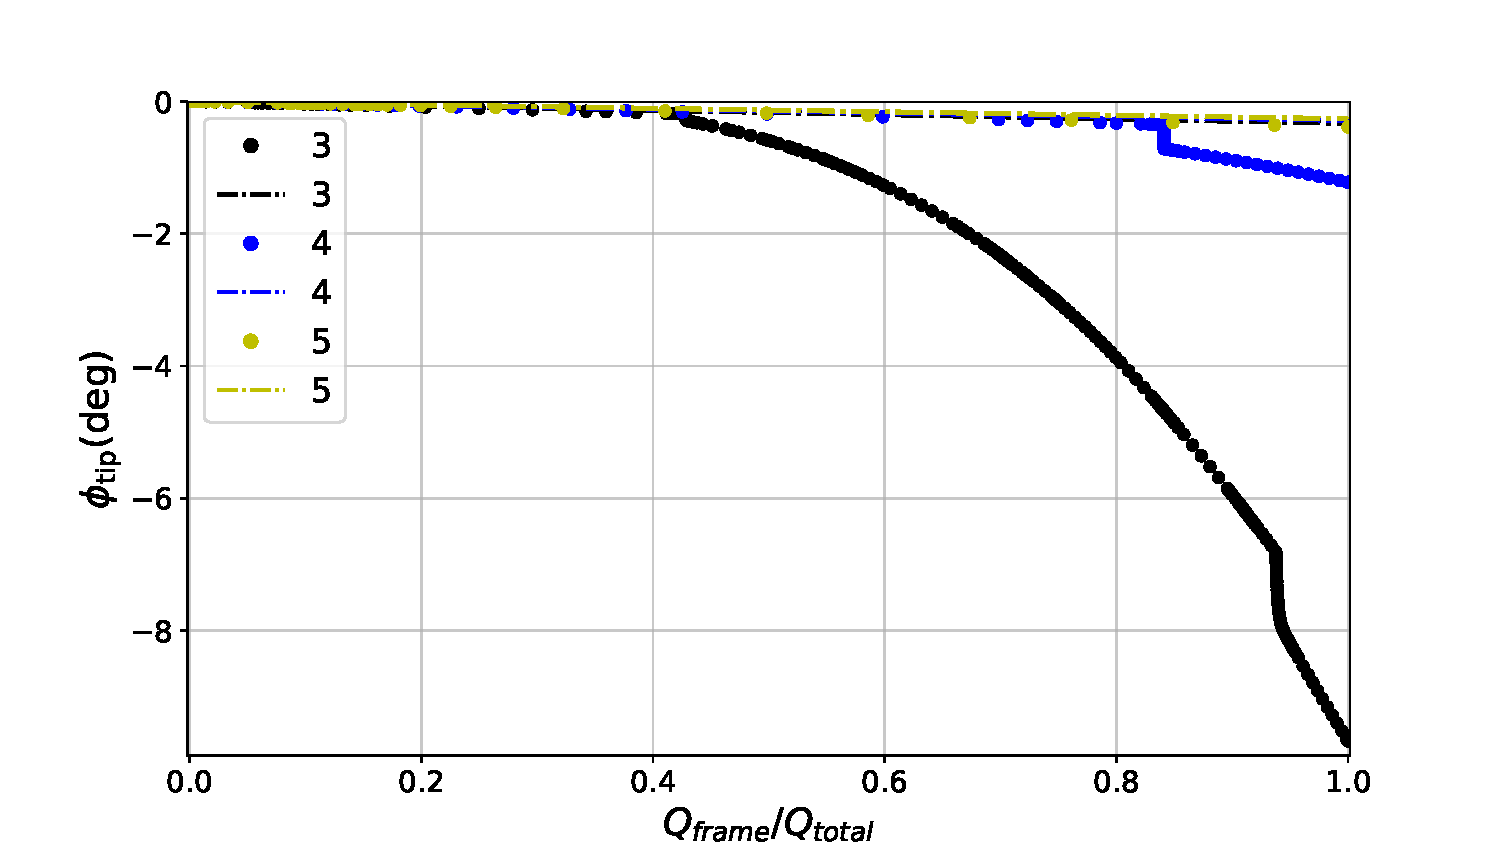
\includegraphics[width=0.8 \textwidth]{figures/result-sim/M/force_displacement-far-1200N}
      \caption[Displacement-force curve for various values of the number of unit cells in the transversal direction]{Displacement-force curve for various values of the number of unit cells in the transversal direction $M$. For all the cases shown, the load introduction point was located in the middle of the upper flange of the tip rib and its magnitude was equal to -1200 N.}\label{fig:forceDisplacement-far-M}
    \end{figure}

    % Now with N
    \clearpage
    The effects of the variation of the number of unit cells in the spanwise direction $N$, parameter responsible of the wing-box length, are investigated next. The results from the parametric study carried out are shown in Table \ref{tab:para_N}. The displacement-force curve for the simulations carried out is shown in Figure \ref{fig:forceDisplacement-far-N}. It can be seen that the bigger the wing-box length, the earlier that the buckling of the lattices cause the collapse of the structure.

    \begin{table}[!htpb] %Results of N
      \centering
      \begin{tabular}{|l|l|l|l|l|l|l|l|l|}
      \hline
      $N$ & $\phi_{\mathrm{tip}}$ (deg) & $e(\phi_{\mathrm{tip}}) (\%)$ & $\tilde{\phi}_{\mathrm{tip}}$ (deg) & $e(\tilde{\phi}_{\mathrm{tip}}) (\%)$ & $v_{\mathrm{max}}$ & $\hat{z}_{v_{\mathrm{max}}}$ & $\hat{x}_{v_{\mathrm{max}}}$ \\ \hline
      7 & -0.215 & 13.74 & -0.165 & -18.212 & -1.182 & 1 & 0.971 \\ \hline
      8 & -1.596 & 14.222 & -0.203 & -18.444 & -14.267 & 1 & 0.334 \\ \hline
      9 & -3.419 & 9.419 & -0.231 & -12.654 & -20.361 & 1 & 0.324 \\ \hline
      10 & -10.516 & 7.756 & -0.27 & -10.353 & -61.202 & 1 & 0.971 \\ \hline
      11 & -22.16 & 6.466 & -0.321 & -8.819 & -138.196 & 1 & 0.971 \\ \hline
      12 & -31.558 & 5.316 & -0.374 & -7.222 & -207.335 & 1 & 0.971 \\ \hline
      \end{tabular}
      \caption[Results from the parametric study on the number of unit cells in the spanwise direction]{Results from the parametric study on the number of unit cells in the spanwise direction $M$. The results show the mean twist at the tip of the wing-box for the Abaqus nonlinear simulation $\phi_{\mathrm{tip}}$ and for the linear simulation $\tilde{\phi}_{\mathrm{tip}}$. The maximum relative error of the mean calculation, expressed as percentage, for these two magnitudes is $e(\phi_{\mathrm{tip}})$ and $e(\tilde{\phi}_{\mathrm{tip}})$, respectively. The table also shows the maximum vertical displacement $v_{\mathrm{max}}$ among all the mesh nodes located on the upper skin of the wing-box and the dimensionless position in the spanwise direction $\hat{x}_{v_{\mathrm{max}}}$ and in the chordwise direction $\hat{z}_{v_{\mathrm{max}}}$ of the node that shows $v = v_{\mathrm{max}}$.}
      \label{tab:para_N}
    \end{table}

    \begin{figure}[!htpb] %force_displacement-far
      \centering
      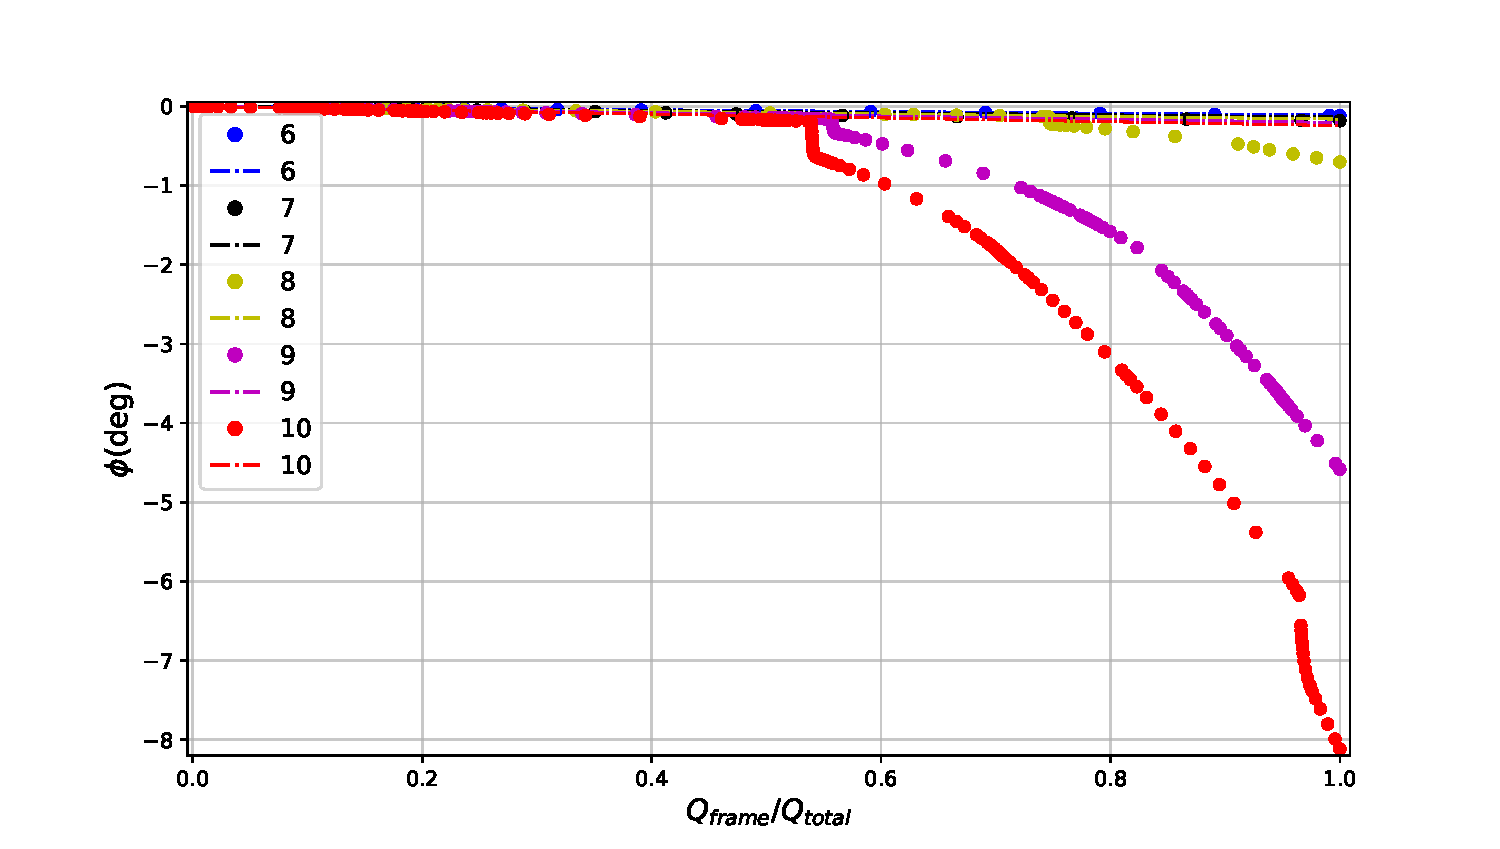
\includegraphics[width=0.8 \textwidth]{figures/result-sim/N/force_displacement-far}
      \caption[Displacement-force curve for various values of the number of unit cells in the spanwise direction]{Displacement-force curve for various values of the number of unit cells in the spanwise direction $N$. For all the cases shown, the load introduction point was located in the middle of the upper flange of the tip rib and its magnitude was equal to -700 N.}\label{fig:forceDisplacement-far-N}
    \end{figure}

    %Second stage of the buckling
    In Figure \ref{fig:forceDisplacement-far-N}, a second change in the slope of the curve for the cases of $N = 10$ and $N = 11$ can be seen. This happens when, as explained in Section \ref{sec:generalResponseCharact_results_sim}, the buckling phenomena progresses from the ligaments at the root to be more generalized in other parts of the structure. This characteristic can be seen in Figure \ref{fig:N10-UR}, where the response of the structure for the case of $N = 10$ and load fraction of $81\%$ is shown.

    \begin{figure}[!htpb] %UR for N = 10
      \centering
      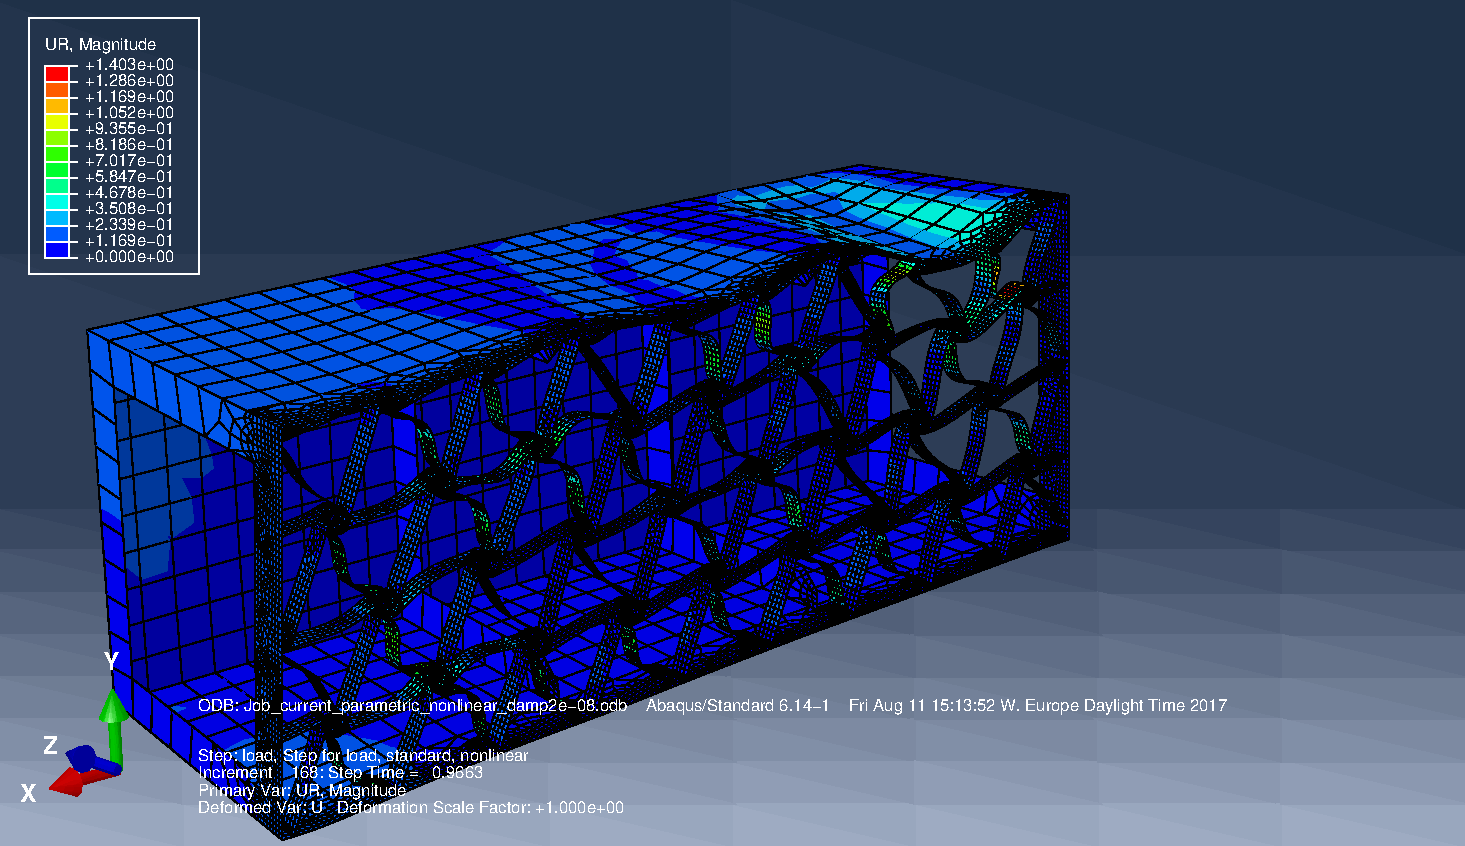
\includegraphics[width=0.8 \textwidth]{figures/result-sim/N/10}
      \caption[Colour contour showing the total rotational displacement when the fraction of load applied equals to 81\% of the prescribed load (700 N) and $N = 10$]{Colour contour showing the total rotational displacement when the fraction of load applied equals to 81\% of the prescribed load (700 N) and $N = 10$. The plot shows how the buckling phenomena is generalized for the whole chiral structure.}\label{fig:N10-UR}
    \end{figure}

    When plotting the force that makes the structure to collapse against the corresponding wing-box length, the Figure \ref{fig:force_N} is produced. This graphic shows that, for example, a force of 300 N is required to induce the collapse of a wing-box with length equal to 1000 mm.

    \begin{figure}[!htpb] %force_plot
      \centering
      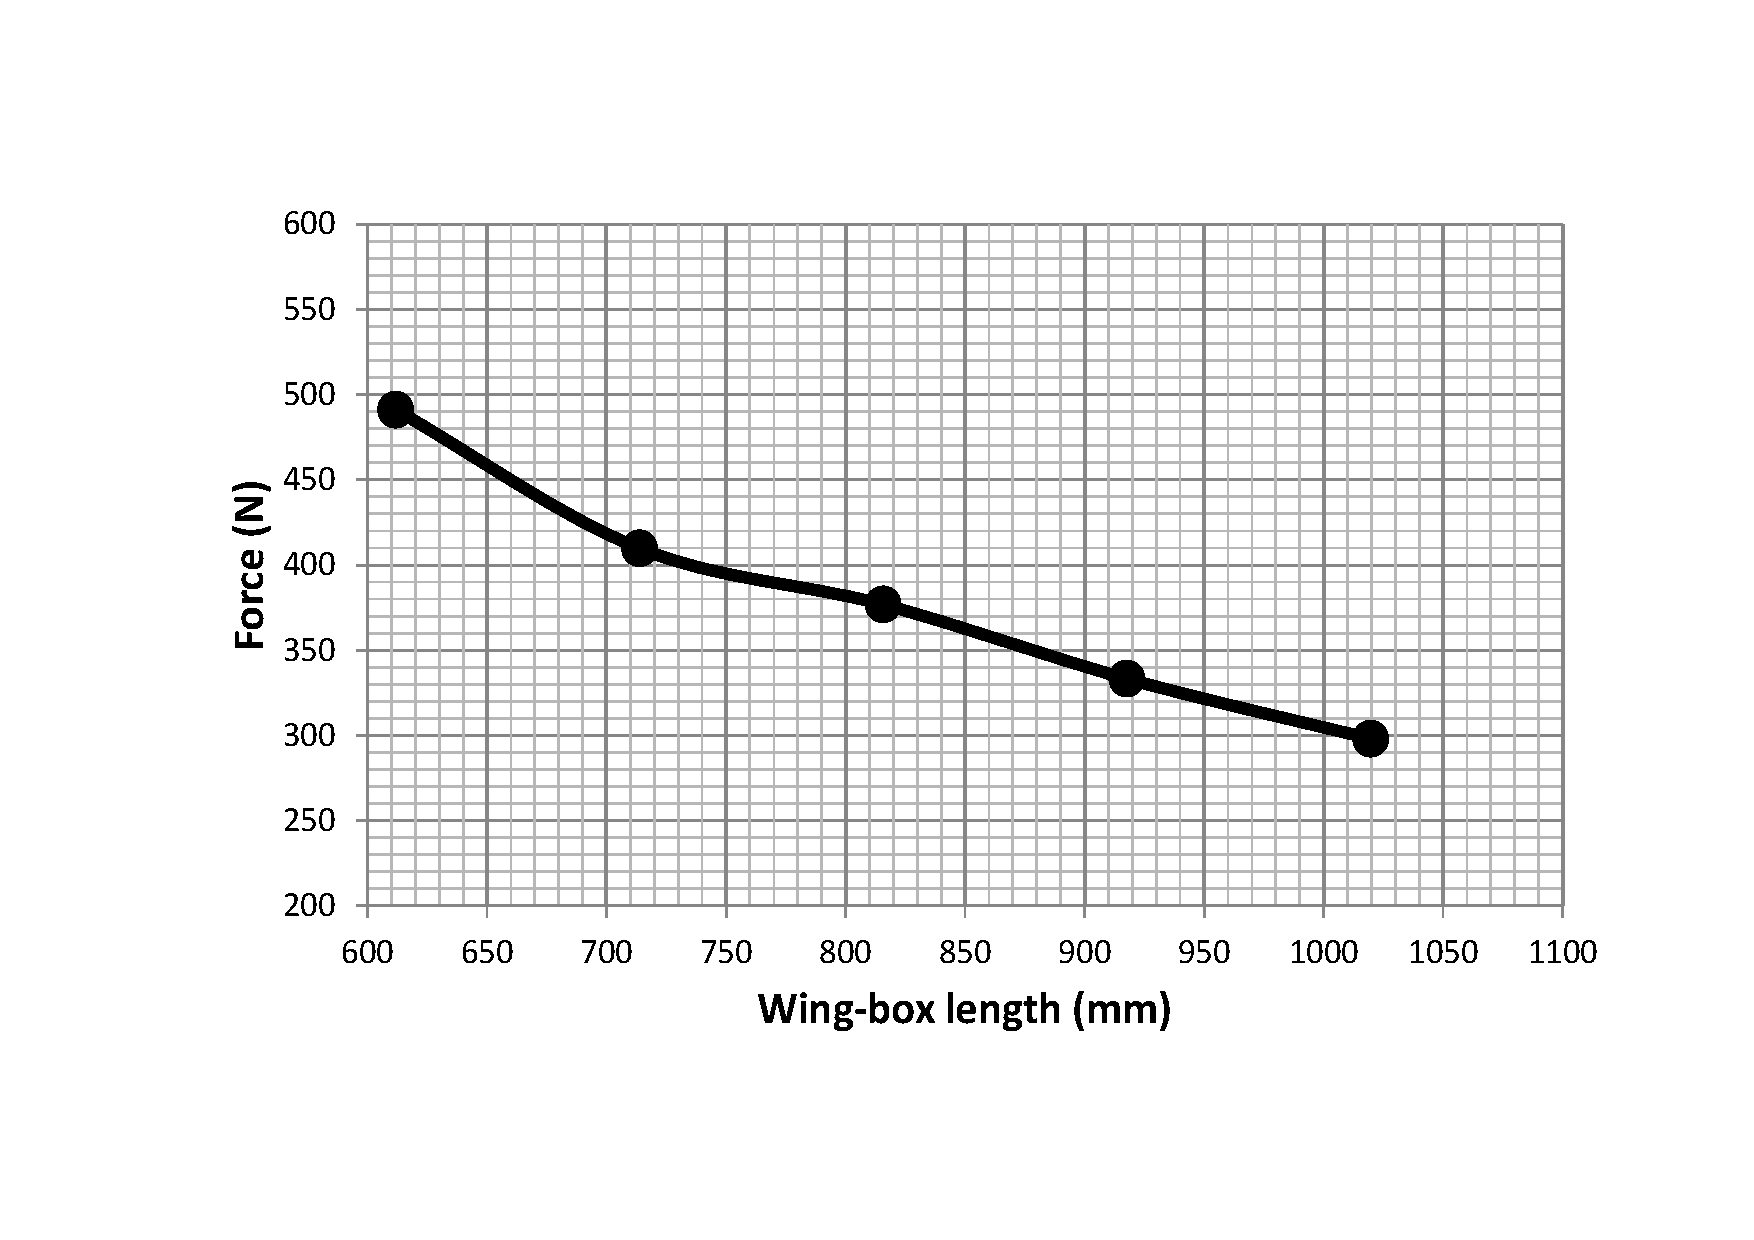
\includegraphics[width=0.8 \textwidth]{figures/result-sim/N/force_N}
      \caption[Force that induces the structure to collapse as a function of the wing-box length]{Force that induces the structure to collapse as a function of the wing-box length.}\label{fig:force_N}
    \end{figure}

  \clearpage
  \subsection{Chiral lattice parameters} \label{subsec:chiral_para}

    In the present subsection, the following parameters of the chiral lattice structure are varied and its effect of the system response is shown:
    %
    \begin{itemize}
      \item Chiral node depth \chiB
      \item Chiral node radius \chir
      \item Chiral lattice thickness \chit
      \item Chiral ligament half length \chiL
      \item Dimensionless ligament eccentricity \chie
    \end{itemize}

    \subsubsection{Dimensionless chiral ligament eccentricity $\epsilon_{\mathrm{chi}}$}
      % \ref{fig:result-sim/eccen/force_displacement-far}
      % In Figure \ref{fig:result-sim/eccen/0coma1-700N} it can be seen than the excesive eccentricity of the ligaments keep them from causing the collapse of the structure

      The first of the chiral structure parameters that is studied is the ligament eccentricity $e_{\mathrm{chi}}$, in its dimensionless form $\epsilon_{\mathrm{chi}}$. The geometrical meaning of this parameter can be seen in the sketch shown in Figure \ref{fig:lattice-internalParameters}. The numeric results from the simulations carried out can be seen in Table \ref{tab:para_e}.

      \begin{table}[!htpb] %Results of chiral thickness
        \centering
        \begin{tabular}{|l|l|l|l|l|l|l|l|l|}
        \hline
        \chie & $\phi_{\mathrm{tip}}$ (deg) & $e(\phi_{\mathrm{tip}}) (\%)$ & $\tilde{\phi}_{\mathrm{tip}}$ (deg) & $e(\tilde{\phi}_{\mathrm{tip}}) (\%)$ & $v_{\mathrm{max}}$ & $\hat{z}_{v_{\mathrm{max}}}$ & $\hat{x}_{v_{\mathrm{max}}}$ \\ \hline
        0      & -0.372 & 12.092 & -0.182 & -13.82 & -4.147  & 1 & 0.546 \\ \hline
        0.001  & -1.194 & 11.467 & -0.191 & -15.24 & -11.731 & 1 & 0.334 \\ \hline
        0.0015 & -0.703 & 15.571 & -0.16  & -10.22 & -7.122  & 1 & 0.546 \\ \hline
        0.01   & -1.596 & 14.222 & -0.203 & -18.44 & -14.267 & 1 & 0.334 \\ \hline
        0.05   & -1.275 & 14.18  & -0.223 & -18.27 & -12.298 & 1 & 0.334 \\ \hline
        0.1    & -0.282 & 14.065 & -0.229 & -18.3  & -2.044  & 1 & 0.334 \\ \hline
        \end{tabular}
        \caption[Results from the parametric study on the dimensionless chiral ligament eccentricity]{Results from the parametric study on the dimensionless chiral ligament eccentricity \chie. The results show the mean twist at the tip of the wing-box for the Abaqus nonlinear simulation $\phi_{\mathrm{tip}}$ and for the linear simulation $\tilde{\phi}_{\mathrm{tip}}$. The maximum relative error of the mean calculation, expressed as percentage, for these two magnitudes is $e(\phi_{\mathrm{tip}})$ and $e(\tilde{\phi}_{\mathrm{tip}})$, respectively. The table also shows the maximum vertical displacement $v_{\mathrm{max}}$ among all the mesh nodes located on the upper skin of the wing-box and the dimensionless position in the spanwise direction $\hat{x}_{v_{\mathrm{max}}}$ and in the chordwise direction $\hat{z}_{v_{\mathrm{max}}}$ of the node that shows $v = v_{\mathrm{max}}$.}
        \label{tab:para_e}
      \end{table}

      The force-deformation curve for the range of simulations carried out can be seen in Figure \ref{fig:forceDisplacement-far-e}. Here it can be seen that the collapse of the structure occurs for all the cases except for \chie$= 0.1$. The deformation state of the structure for this case can be seen in Figure \ref{fig:e0coma1-UR} that shows how the excessive eccentricity of the ligaments keep them from buckling and causing the structure collapse.

      \begin{figure}[!htpb] %force_displacement-far
        \centering
        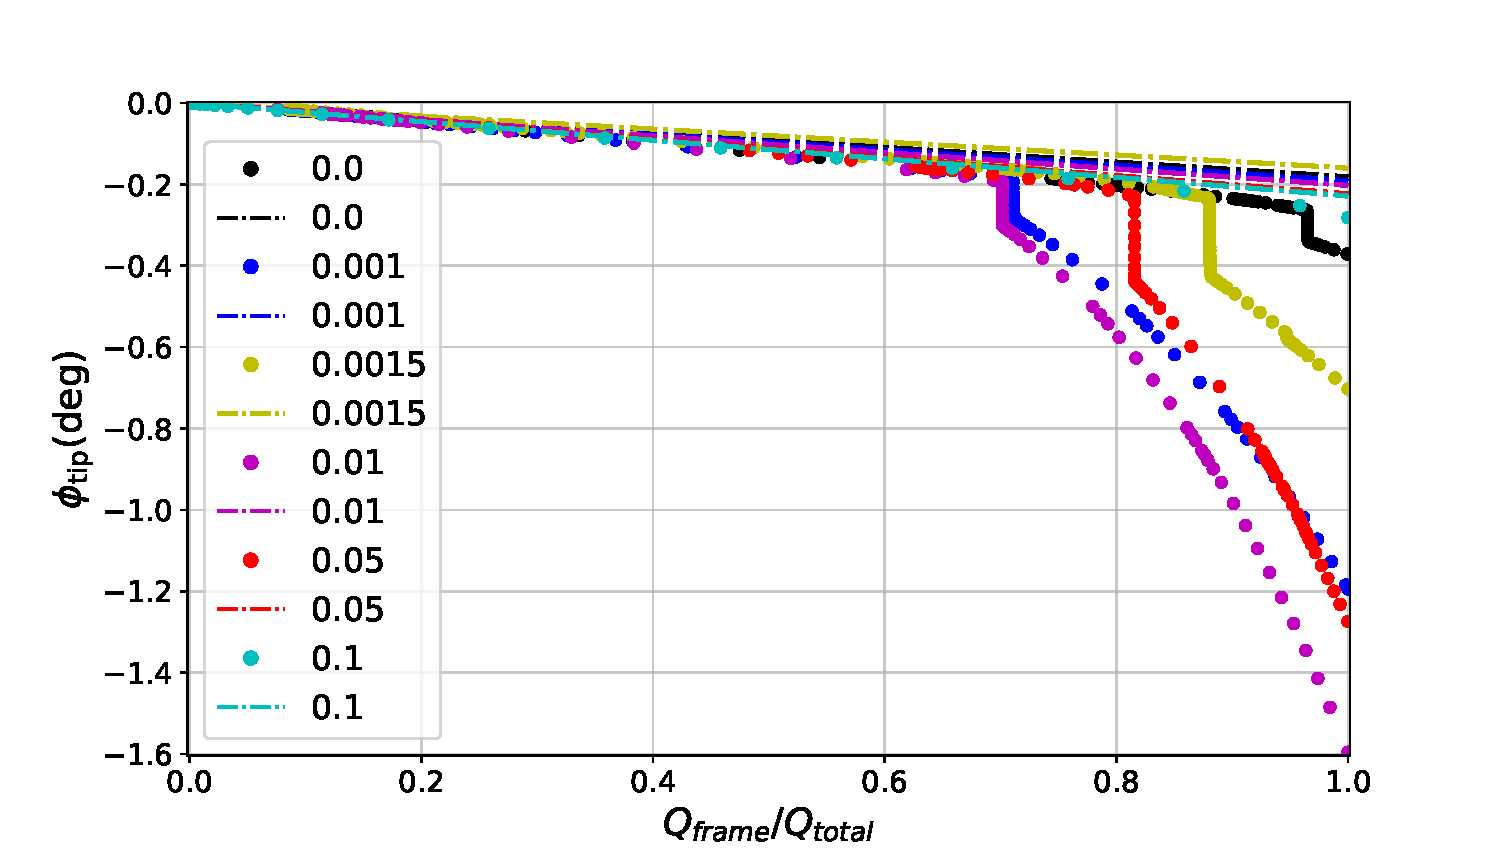
\includegraphics[width=0.8 \textwidth]{figures/result-sim/eccen/force_displacement-far}
        \caption[Displacement-force curve for various values of the dimensionless chiral ligament eccentricity]{Displacement-force curve for various values of the dimensionless chiral ligament eccentricity \chie. The plot shows how the collapse of the structure occurs for all the cases except for \chie$= 0.1$.}\label{fig:forceDisplacement-far-e}
      \end{figure}

      \begin{figure}[!htpb] %UR for e = 0.1
        \centering
        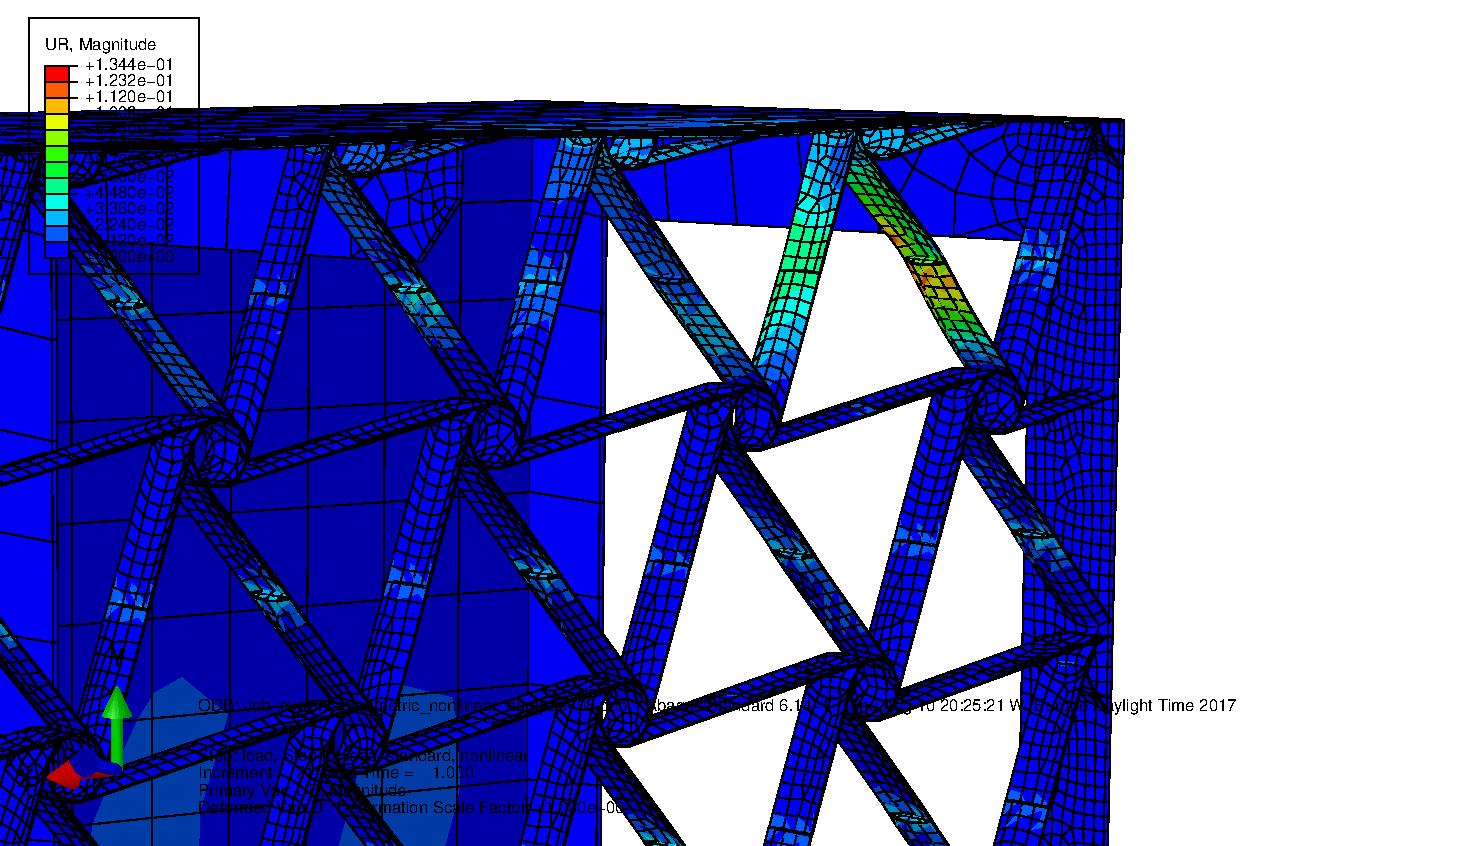
\includegraphics[width=0.6 \textwidth]{figures/result-sim/eccen/0coma1-700N}
        \caption[Colour contour showing the total rotational displacement when the fraction of load applied equals to 100\% of the prescribed load (700 N) and \chie$= 0.1$]{Colour contour showing the total rotational displacement when the fraction of load applied equals to 100\% of the prescribed load (700 N) and \chie$= 0.1$. For this case, the excessive ligament eccentricity at the end of the simulation keeps it from buckling and causing the structure collapse.}
        \label{fig:e0coma1-UR}
      \end{figure}

      The Figure \ref{fig:forceDisplacement-far-e} also shows that the case of \chie$ = 0.0$, that is when the ligaments are flat, is not the case that shows a earlier onset of the instabilities, as it would be expected. Instead, for \chie$ = 0.0$, the structure shows the later onset of the instabilities, when the applied load is 96\% of the prescribed load. On the other hand, the collapse of the structure is triggered when the applied load is 68\% of the prescribed load for the case of \chie$ = 0.001$. This particular behavior is investigated by looking at the deformed plots on the Abaqus visualization module. In Figures \ref{fig:0coma0_UR} and \ref{fig:0coma001_UR} the deformed state of the ligaments at the point when collapse of the structure occurs is shown for the cases of \chie$ = 0.0$ and \chie$ = 0.001$, respectively. It can be seen that the buckling mechanism in the ligaments changes between the two cases. In particular, it can be seen that for \chie$ = 0.0$ the onset of the instabilities induces some rotation to the lattice nodes located on the upper part. The particular geometry of the model is believed to be the reason behind this differences in the appearance of buckling at the ligaments at the root. 
      %
      % \begin{figure}[!htpb] %plot with different forces that make the structure to collapse for e
      %   \centering
      %   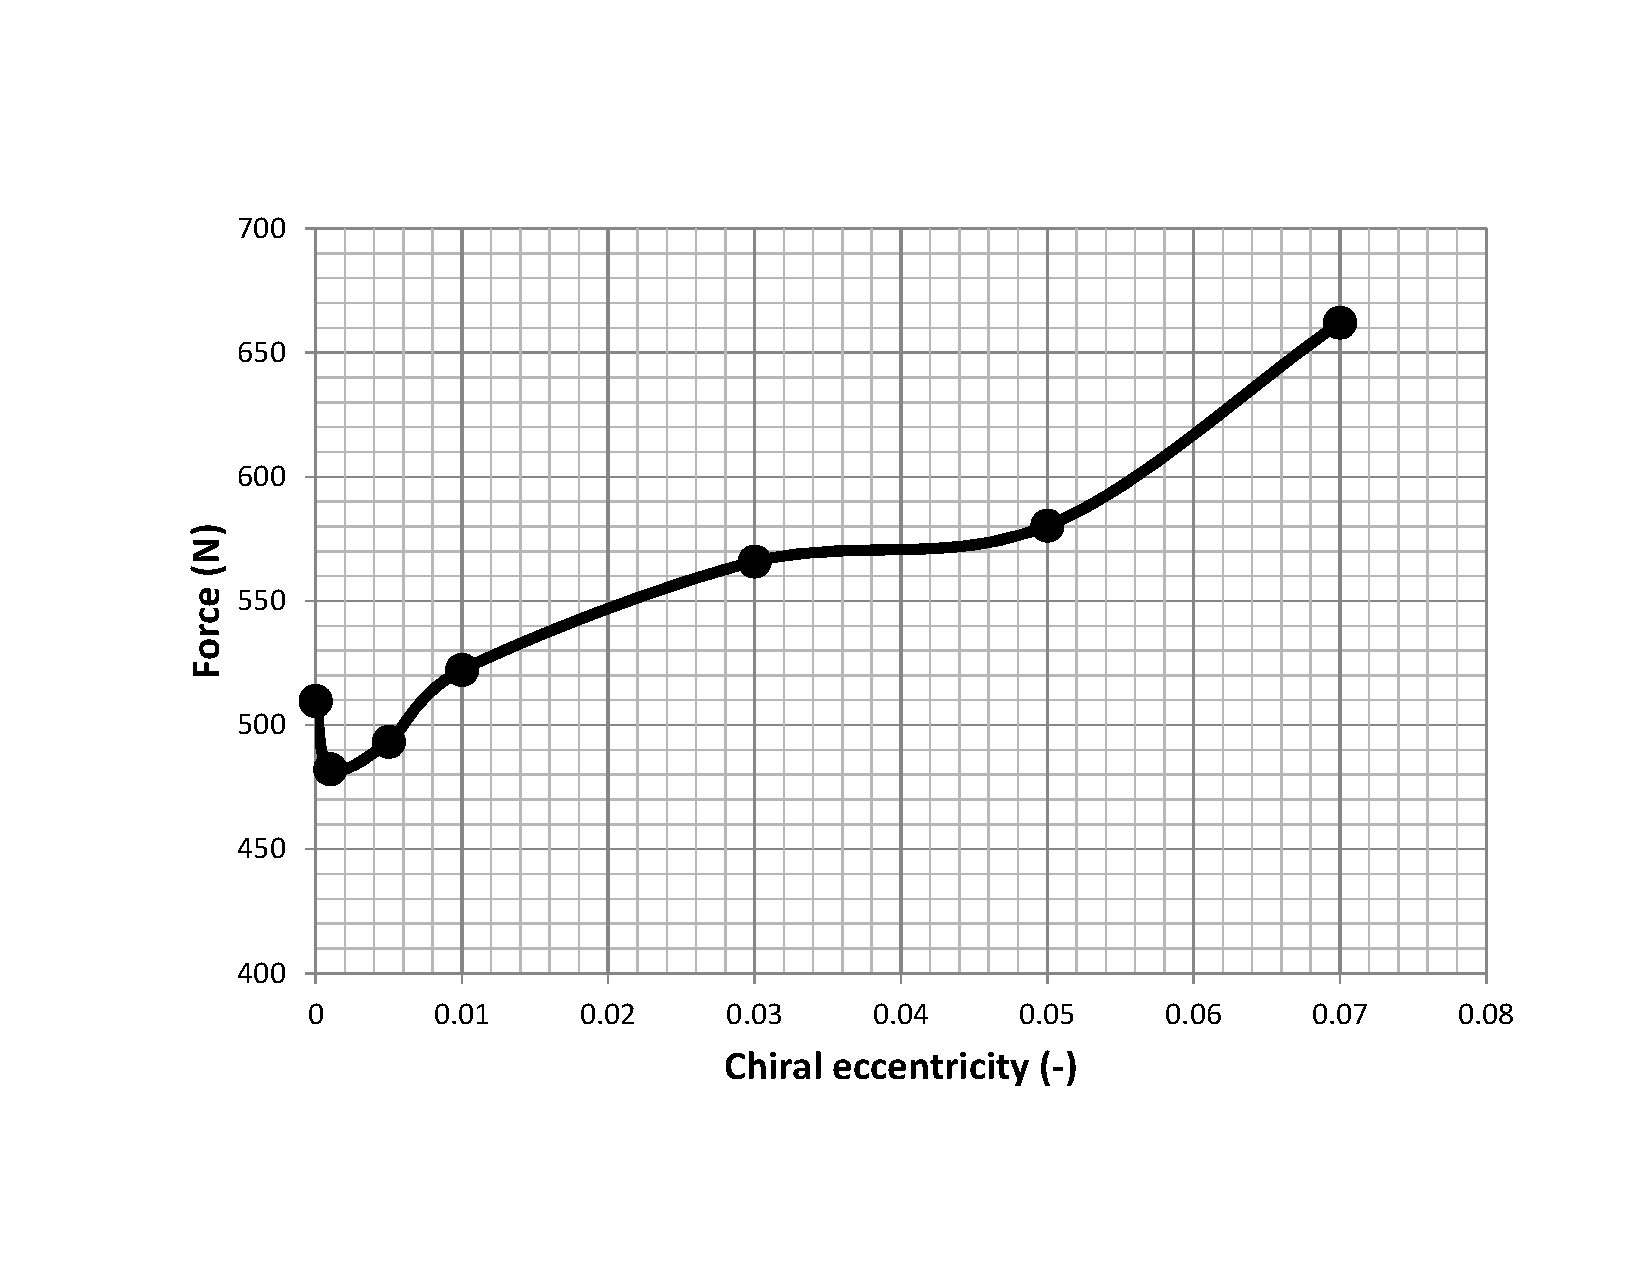
\includegraphics[width=0.8 \textwidth]{figures/result-sim/eccen/force_e}
      %   \caption[Force that induces the structure to collapse as a function of the chiral ligament eccentricity]{Force that induces the structure to collapse as a function of the chiral ligament eccentricity \chie. It can be seen that the .}
      %   \label{fig:force_e}
      % \end{figure}

      \begin{figure}[!htpb] %plot with different forces that make the structure to collapse for e
        \centering
        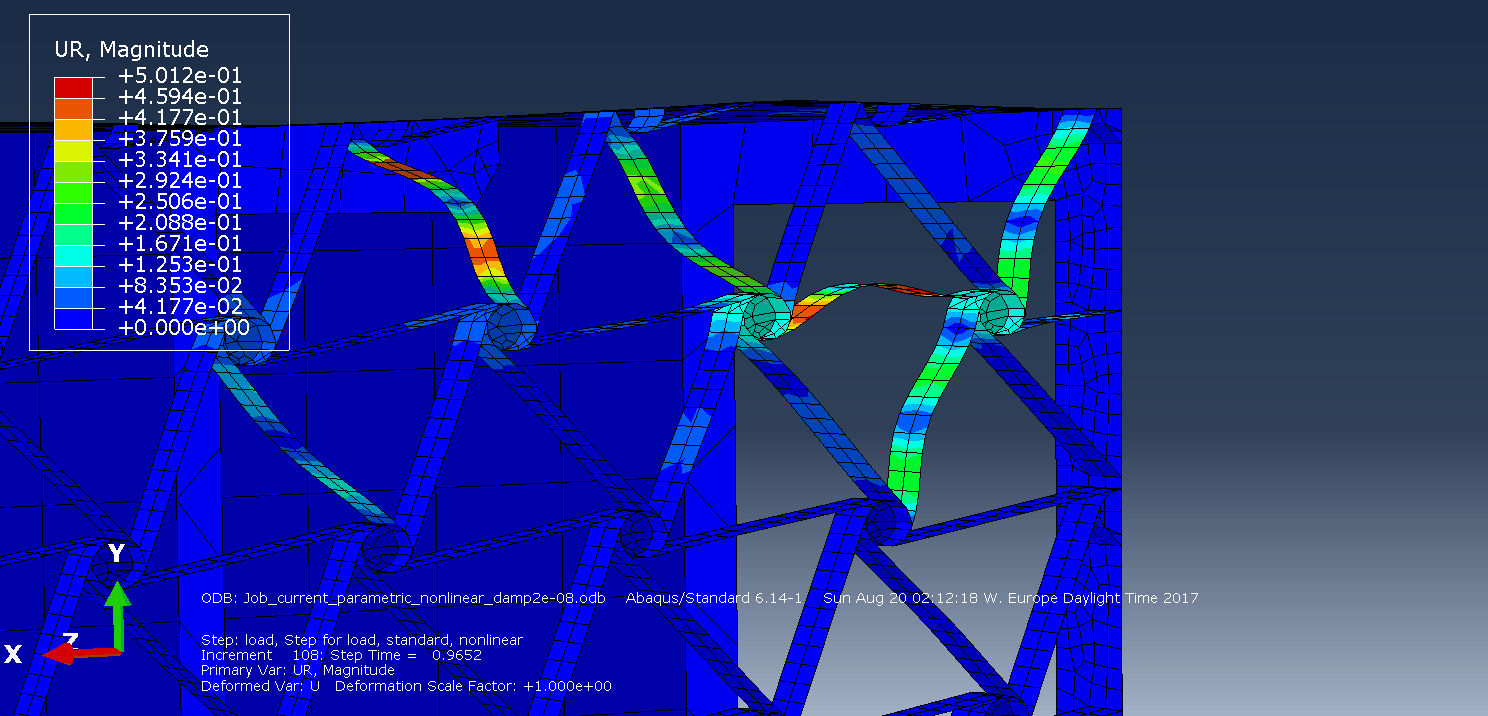
\includegraphics[width=0.7 \textwidth]{figures/result-sim/eccen/0coma0_UR}
        \caption[Colour contour showing the total rotational displacement when the fraction of load applied equals to 96\% of the prescribed load (700 N) and \chie$= 0.0$]{Colour contour showing the total rotational displacement when the fraction of load applied equals to 96\% of the prescribed load (700 N) and \chie$= 0.0$. In this case, the onset of the instabilities affect the rotation of the lattice nodes, in particular. There are two ligaments on the upper part that remain undeformed.}
        \label{fig:0coma0_UR}
      \end{figure}

      \begin{figure}[!htpb] %plot with different forces that make the structure to collapse for e
        \centering
        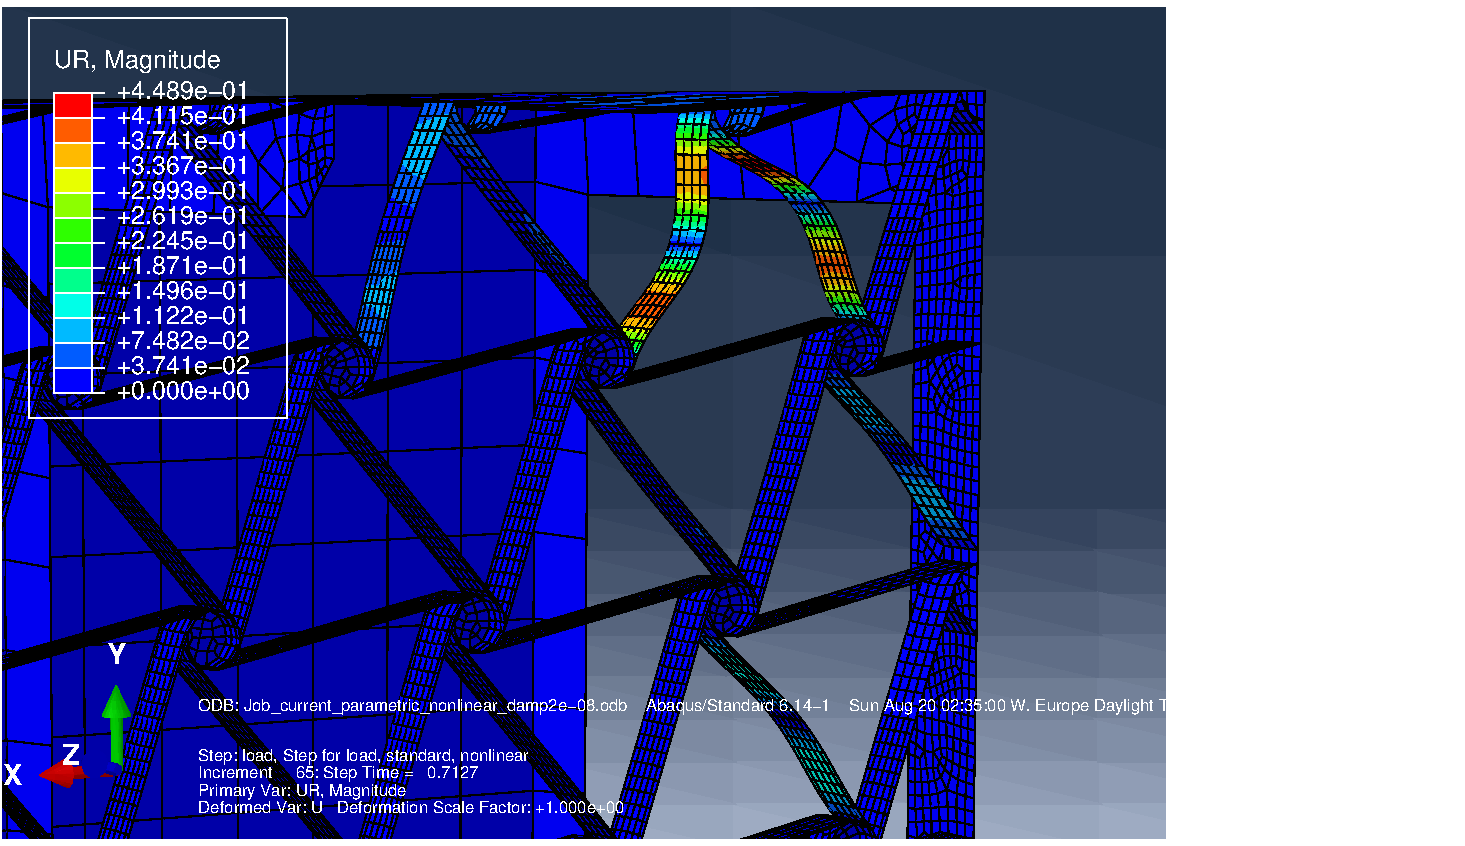
\includegraphics[width=0.7 \textwidth]{figures/result-sim/eccen/0coma001_UR}
        \caption[Colour contour showing the total rotational displacement when the fraction of load applied equals to 71\% of the prescribed load (700 N) and \chie$= 0.001$]{Colour contour showing the total rotational displacement when the fraction of load applied equals to 71\% of the prescribed load (700 N) and \chie$= 0.001$.}
        \label{fig:0coma001_UR}
      \end{figure}

    \clearpage
    \subsubsection{Chiral node depth $B_{\mathrm{chi}}$}
      %
      % \ref{fig:result-sim/B/force_displacement-far}
      % The larger the chiral node depth, the bigger surface on the
      % The collapse point moves backwards as the $B_{\mathrm{chi}}$ increases. However, the bigger $B_{\mathrm{chi}}$, the more abrupt the collapse is.
      % It Figure \ref{fig:result-sim/B/30_UR1} the rotation $UR_1$ of the mesh elements around the $x$ direction can be seen for the case of \B$= 30$mm at the moment when collapse of the structure ocurrs. The value of this magnitude in this area is approximatelly the double to the corresponding one when \B$= 10$mm which can be seen in Figure \ref{fig:result-sim/B/10_UR1}

      The numeric results from the parametric analysis on the chiral node depth \chiB can be seen in Table \ref{tab:para_B}. The geometrical meaning of this parameter can be seen in the sketch shown in Figure \ref{fig:lattice-internalParameters}. The displacement-force curve can be seen in Figure \ref{fig:forceDisplacement-far-B} for various values of $B$.

      The Figure \ref{fig:30_UR1} shows a colour contour plot representing the rotation $u$ around the $x$ direction of the mesh elements located on the upper skin of the wing-box and close to the root. This is represented for the case of \chiB $= 30$ mm, at the moment when collapse of the structure occurs which is at $86\%$ of the prescribed load and in the area where local deformation of the skin appear. Examination of the plot arises that the value of $u$ in this area is approximately double to the case of \chiB$= 10$ mm, which can be seen in Figure \ref{fig:10_UR1}. This shows that the bigger \chiB is, the more area is affected by the ligaments deformation when buckling occurs and the greater the local deformation is.

      When plotting the force that makes the structure to collapse against the corresponding value of chiral node depth depth \chiB, the Figure \ref{fig:force_B} is produced.

      \begin{table}[!htpb] %Results of B
        \centering
        \begin{tabular}{|l|l|l|l|l|l|l|l|l|}
        \hline
        \chiB & $\phi_{\mathrm{tip}}$ (deg) & $e(\phi_{\mathrm{tip}}) (\%)$ & $\tilde{\phi}_{\mathrm{tip}}$ (deg) & $e(\tilde{\phi}_{\mathrm{tip}}) (\%)$ & $v_{\mathrm{max}}$ & $\hat{z}_{v_{\mathrm{max}}}$ & $\hat{x}_{v_{\mathrm{max}}}$ \\ \hline
        10 & -1.399 & 11.421 & -0.217 & -15.359 & -12.735 & 1 & 0.334 \\ \hline
        20 & -1.596 & 14.222 & -0.203 & -18.444 & -14.267 & 1 & 0.334 \\ \hline
        30 & -0.707 & 16.454 & -0.216 & -24.477 & -7.975  & 1 & 0.334 \\ \hline
        \end{tabular}
        \caption[Results from the parametric study on chiral node depth]{Results from the parametric study on chiral node depth \chiB. The results show the mean twist at the tip of the wing-box for the Abaqus nonlinear simulation $\phi_{\mathrm{tip}}$ and for the linear simulation $\tilde{\phi}_{\mathrm{tip}}$. The maximum relative error of the mean calculation, expressed as percentage, for these two magnitudes is $e(\phi_{\mathrm{tip}})$ and $e(\tilde{\phi}_{\mathrm{tip}})$, respectively. The table also shows the maximum vertical displacement $v_{\mathrm{max}}$ among all the mesh nodes located on the upper skin of the wing-box and the dimensionless position in the spanwise direction $\hat{x}_{v_{\mathrm{max}}}$ and in the chordwise direction $\hat{z}_{v_{\mathrm{max}}}$ of the node that shows $v = v_{\mathrm{max}}$.}
        \label{tab:para_B}
      \end{table}

      \begin{figure}[!htpb] %force_displacement-far
        \centering
        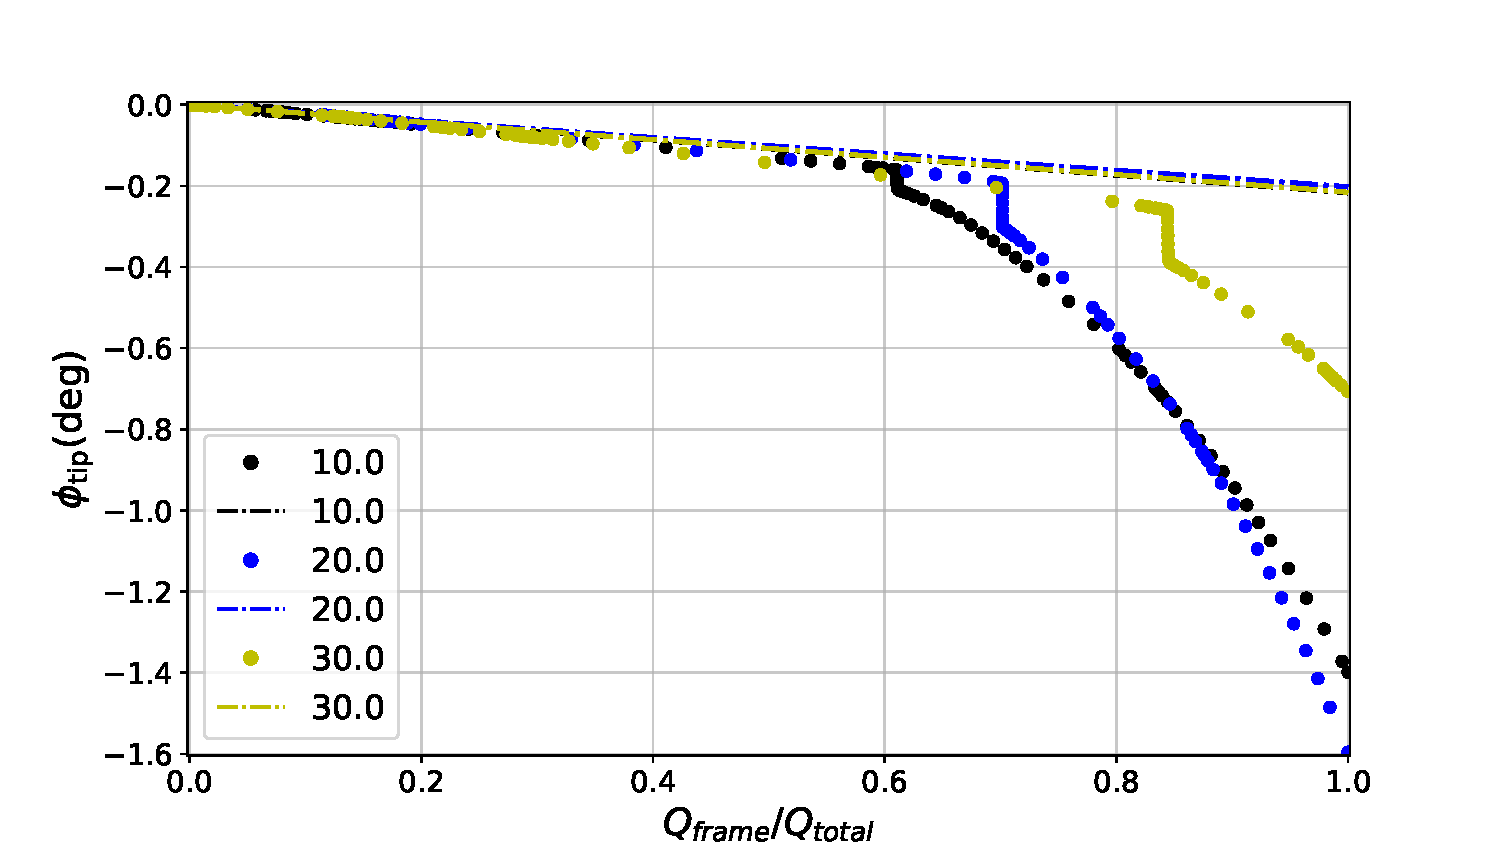
\includegraphics[width=0.8 \textwidth]{figures/result-sim/B/force_displacement-far}
        \caption[Displacement-force curve for various values of the dimensionless chiral node depth]{Displacement-force curve for various values of the dimensionless chiral node depth \chiB. Results show how the bigger the node depth \chiB is, the later the collapse of the structure occurs but the more abrupt is its.}\label{fig:forceDisplacement-far-B}
      \end{figure}

      \begin{figure}[!htpb] %UR for B = 30
        \centering
        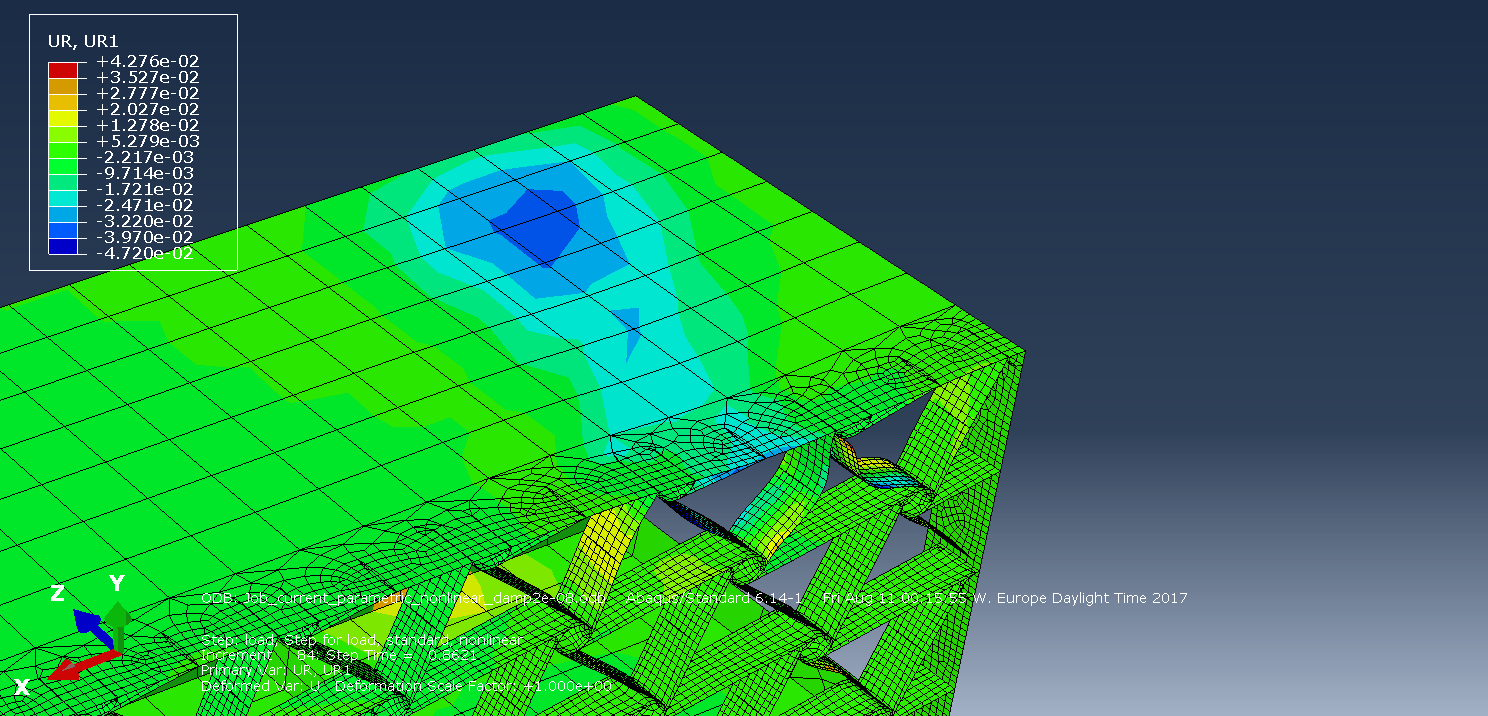
\includegraphics[width=0.8 \textwidth]{figures/result-sim/B/30_UR1}
        \caption[Colour contour showing the total rotational displacement when the fraction of load applied equals to 86\% of the prescribed load (700 N) and \chiB$= 30$ mm]{Colour contour showing the total rotational displacement when the fraction of load applied equals to 86\% of the prescribed load (700 N) and \chiB$= 30$ mm. The plot shows a colour contour with the value of the rotational displacement $u$ around the $x$ direction at the moment in which the structure collapses. In the area where the local deformation occurs, the value of $u$ is approximately equal to $-0.033$ rad.}
        \label{fig:30_UR1}
      \end{figure}

      \begin{figure}[!htpb] %UR for B = 10
        \centering
        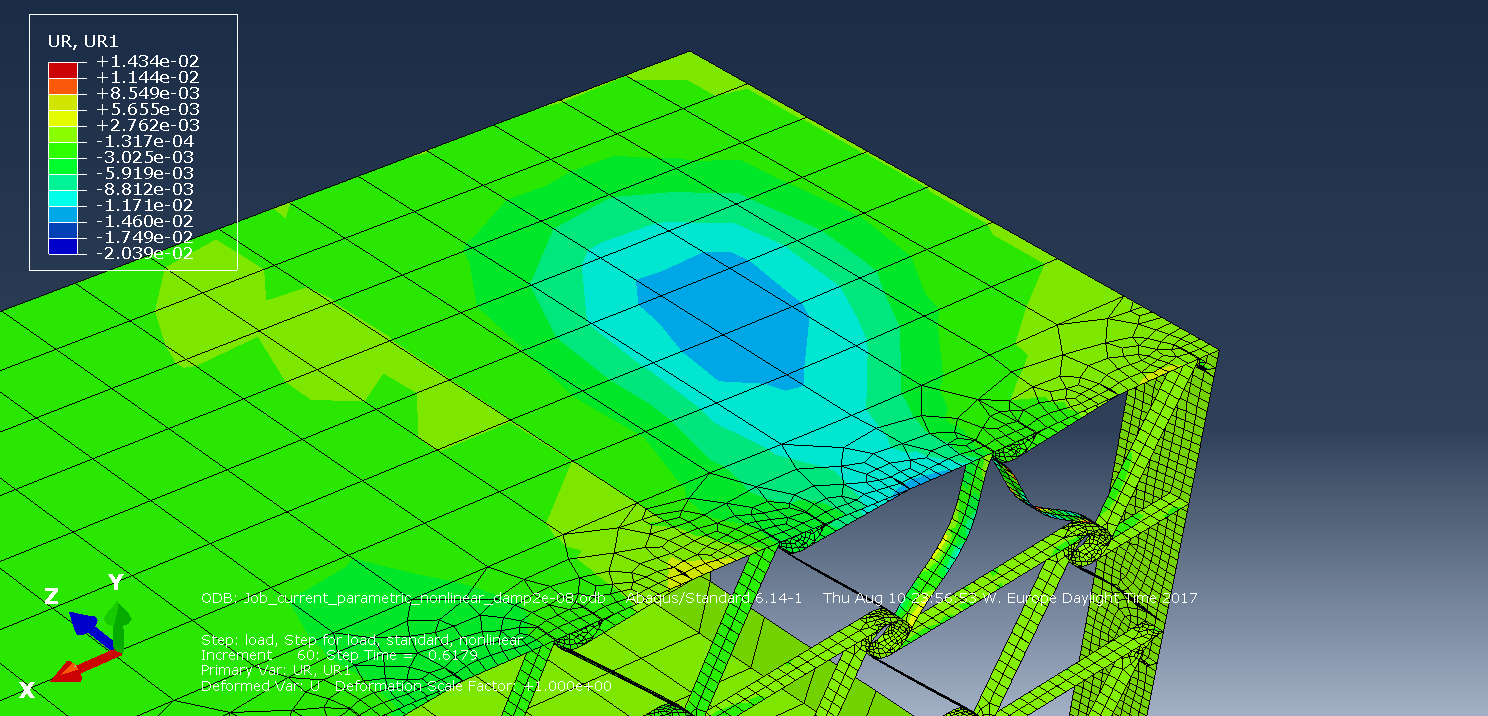
\includegraphics[width=0.8 \textwidth]{figures/result-sim/B/10_UR1}
        \caption[Colour contour showing the total rotational displacement when the fraction of load applied equals to 62\% of the prescribed load (700 N) and \chiB$= 10$ mm]{Colour contour showing the total rotational displacement when the fraction of load applied equals to 62\% of the prescribed load (700 N) and \chiB$= 10$ mm. The plot shows a colour contour with the value of the rotational displacement $u$ around the $x$ direction at the moment in which the structure collapses. In the area where the local deformation occurs, the value of $u$ is approximately equal to $-0.015$ rad.}
        \label{fig:10_UR1}
      \end{figure}

      \begin{figure}[!htpb] %force_plot
        \centering
        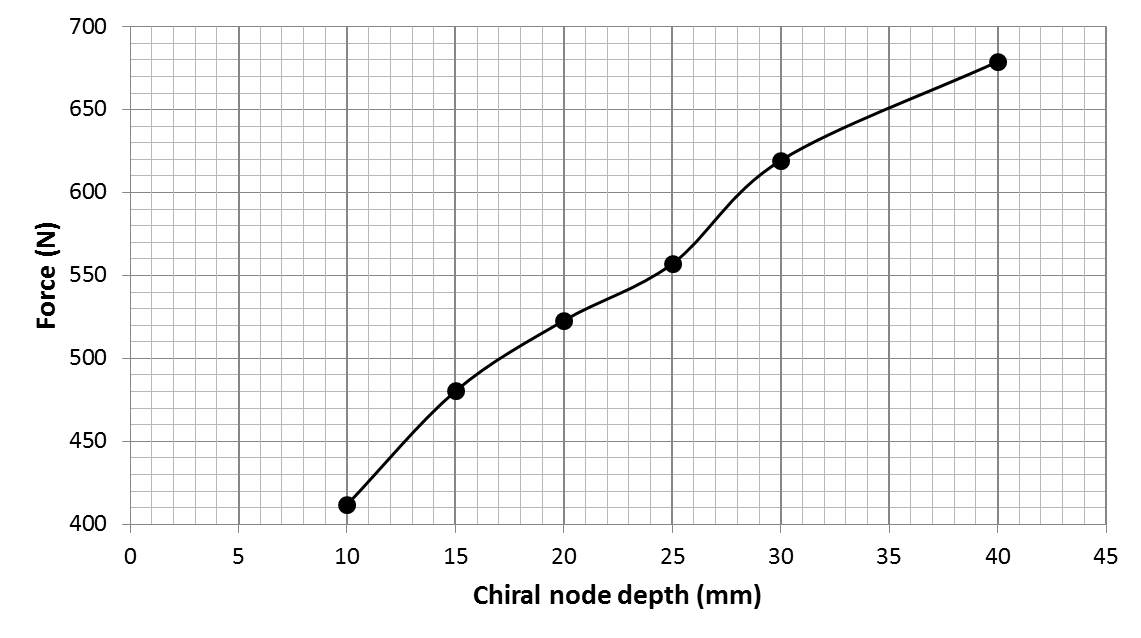
\includegraphics[width=0.8 \textwidth]{figures/result-sim/B/force_B}
        \caption[Force that induces the structure to collapse as a function of the chiral node depth]{Force that induces the structure to collapse as a function of the chiral node depth \chiB.}\label{fig:force_B}
      \end{figure}

    \clearpage
    \subsubsection{Chiral node radius $r_{\mathrm{chi}}$}
      %
      % Ranges: 7.5, 10, 12.5, 15, 17.5, 20
      % \ref{fig:result-sim/r/force_displacement-far}
      % For \r = 5, an error in the ligaments is found. There is interference between the mesh elemnents located at different ligaments that are joined at one node.
      % For \r$= 12.5$mm, the buckling ligaments are located at the root, as it can be seen in Figure \ref{fig:result-sim/r/12coma5-UR}. However, for the case of \r$= 17.5$mm, buckling do not ocurr on the ligaments located at the root but in those located just after the inner rib located closer to the root, with smaller $x$. This explains the characteristic seen in Figure \ref{fig:result-sim/r/force_displacement-far} for the case of \r$= 17.5$mm which breaks the trend followed by values \r$< 17.5$mm.

      A parametric study on different values of the chiral node radius \chir is presented next. The geometrical meaning of this parameter can be seen in the sketch shown in Figure \ref{fig:lattice-internalParameters}. The possible values of \chir are limited by the geometry of the chiral lattice. For values \chir$\le 5$ mm, it is not possible to build the model due to interferences between the different ligaments that joined at each of the nodes. The numeric results from the simulations are presented in Table \ref{tab:para_r}.

      The displacement-force curve obtained from the simulations is shown in Figure \ref{fig:forceDisplacement-far-r}. This curve shows how the structure collapses for all the analysed cases except for \chir$ = 17.5$ mm and \chir$ = 20$ mm. However, for the case of \chir$= 17.5$mm, buckling do not occur on the ligaments located at the root but in those located just after the inner rib located closer to the root, with smaller $x$. This can be seen in Figure \ref{fig:r17coma5-UR}. Then, the chiral node radius \chir value shifts the position of the buckling ligaments that origin the collapse of the structure.

      The variation of the force that makes the structure to collapse as a function of the chiral node radius \chir can be seen in Figure \ref{fig:force_r}. It can be seen that, the smaller the chiral node radius \chir is, the earlier the structure collapse occurs. 

      \begin{table}[!htpb] %Results of r
        \centering
        \begin{tabular}{|l|l|l|l|l|l|l|l|l|}
        \hline
        \chir & $\phi_{\mathrm{tip}}$ (deg) & $e(\phi_{\mathrm{tip}}) (\%)$ & $\tilde{\phi}_{\mathrm{tip}}$ (deg) & $e(\tilde{\phi}_{\mathrm{tip}}) (\%)$ & $v_{\mathrm{max}}$ & $\hat{z}_{v_{\mathrm{max}}}$ & $\hat{x}_{v_{\mathrm{max}}}$ \\ \hline
        7.5 & -1.184 & 13.64 & -0.171 & -10.046 & -11.586 & 1 & 0.331 \\ \hline
        10 & -0.877 & 9.525 & -0.17 & -10.196 & -9.831 & 1 & 0.334 \\ \hline
        12.5 & -0.886 & 9.596 & -0.17 & -10.247 & -10.051 & 1 & 0.337 \\ \hline
        15 & -1.121 & 13.638 & -0.173 & -10.134 & -11.677 & 1 & 0.342 \\ \hline
        17.5 & -0.273 & 9.481 & -0.171 & -10.215 & -4.169 & 1 & 0.568 \\ \hline
        20 & -0.229 & 12.686 & -0.171 & -8.848 & -1.433 & 1 & 1.026 \\ \hline
        \end{tabular}
        \caption[Results from the parametric study on chiral node radius]{Results from the parametric study on chiral node radius \chir. The results show the mean twist at the tip of the wing-box for the Abaqus nonlinear simulation $\phi_{\mathrm{tip}}$ and for the linear simulation $\tilde{\phi}_{\mathrm{tip}}$. The maximum relative error of the mean calculation, expressed as percentage, for these two magnitudes is $e(\phi_{\mathrm{tip}})$ and $e(\tilde{\phi}_{\mathrm{tip}})$, respectively. The table also shows the maximum vertical displacement $v_{\mathrm{max}}$ among all the mesh nodes located on the upper skin of the wing-box and the dimensionless position in the spanwise direction $\hat{x}_{v_{\mathrm{max}}}$ and in the chordwise direction $\hat{z}_{v_{\mathrm{max}}}$ of the node that shows $v = v_{\mathrm{max}}$.}
        \label{tab:para_r}
      \end{table}

      \begin{figure}[!htpb] %force_displacement-far
        \centering
        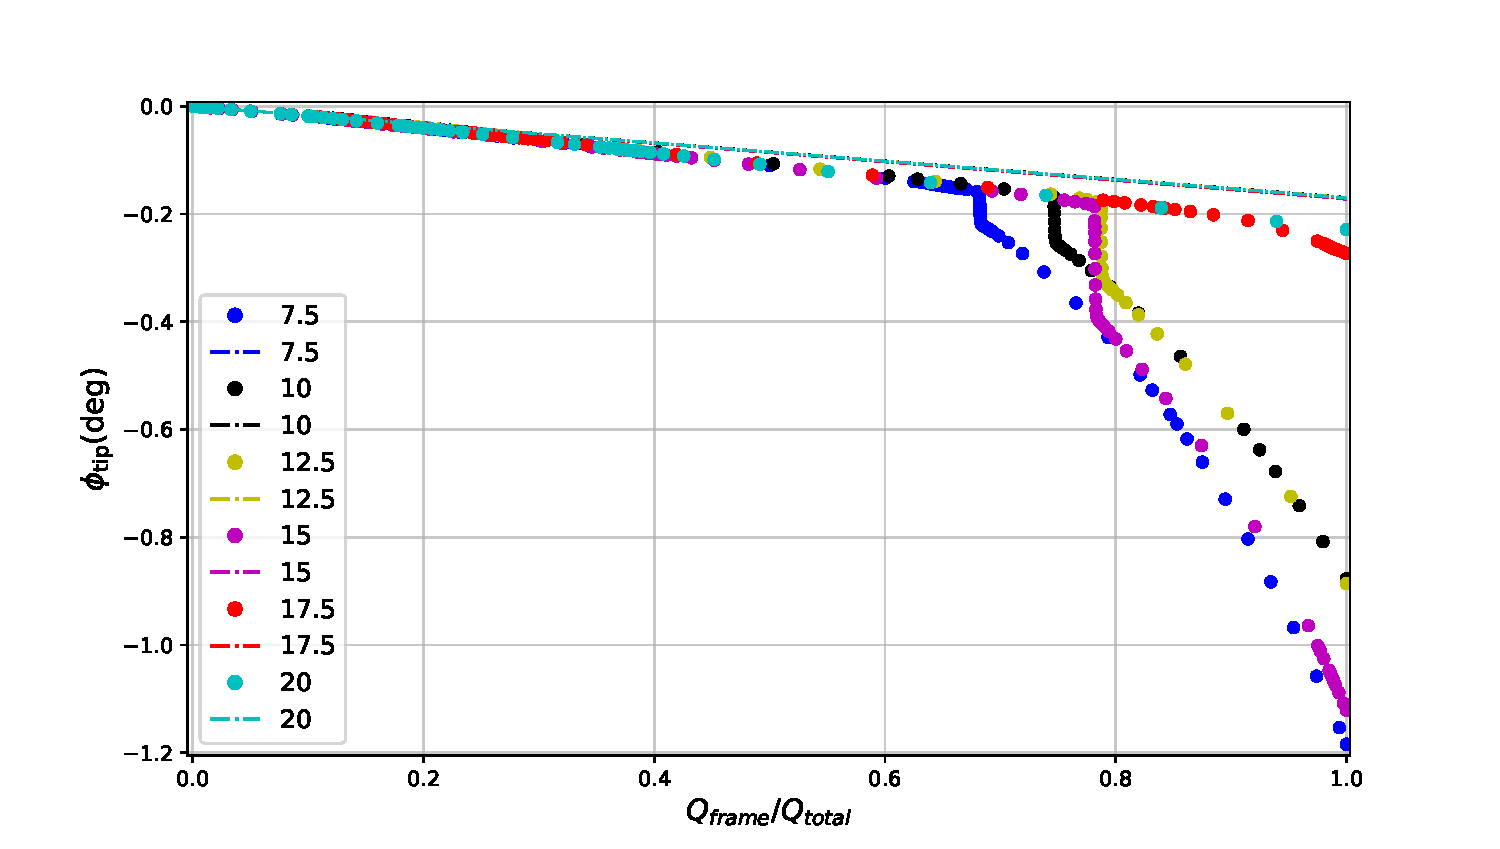
\includegraphics[width=0.8 \textwidth]{figures/result-sim/r/force_displacement-far}
        \caption[Displacement-force curve for various values of the chiral node radius]{Displacement-force curve for various values of the chiral node radius \chir.}\label{fig:forceDisplacement-far-r}
      \end{figure}

      \begin{figure}[!htpb] %UR for r = 17.5
        \centering
        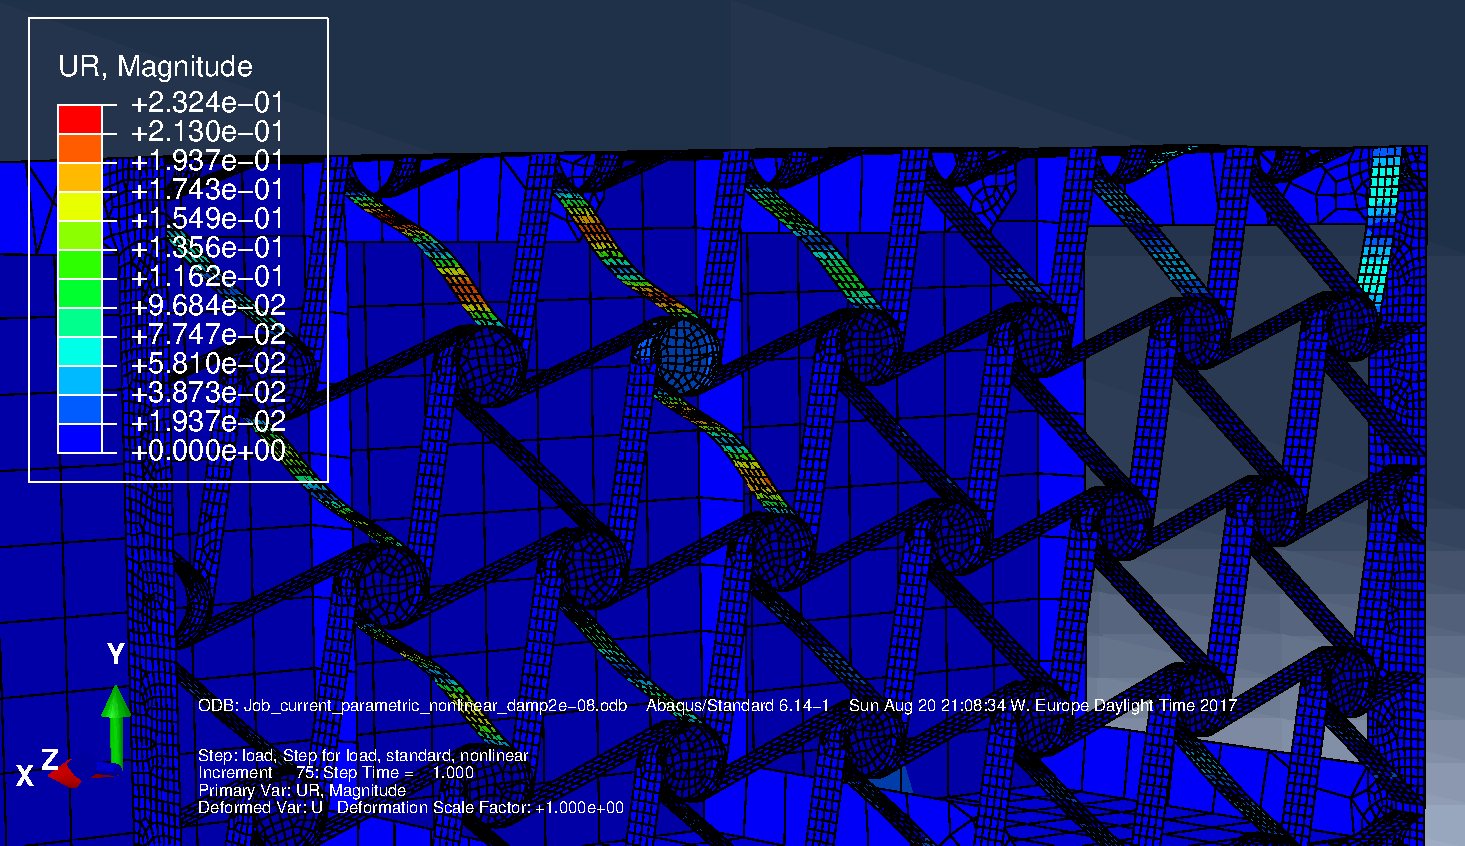
\includegraphics[width=0.8 \textwidth]{figures/result-sim/r/17coma5-UR}
        \caption[Colour contour showing the total rotational displacement when the fraction of load applied equals to 100\% of the prescribed load (700 N) and \chir$ = 17.5$ mm]{Colour contour showing the total rotational displacement when the fraction of load applied equals to 100\% of the prescribed load (700 N) and \chir$ = 17.5$ mm. Here, the excessive value of the chiral node radius \chir makes that the buckled region is moved towards increasing values of $x$.}\label{fig:r17coma5-UR}
      \end{figure}

      \begin{figure}[!htpb] %force_plot
        \centering
        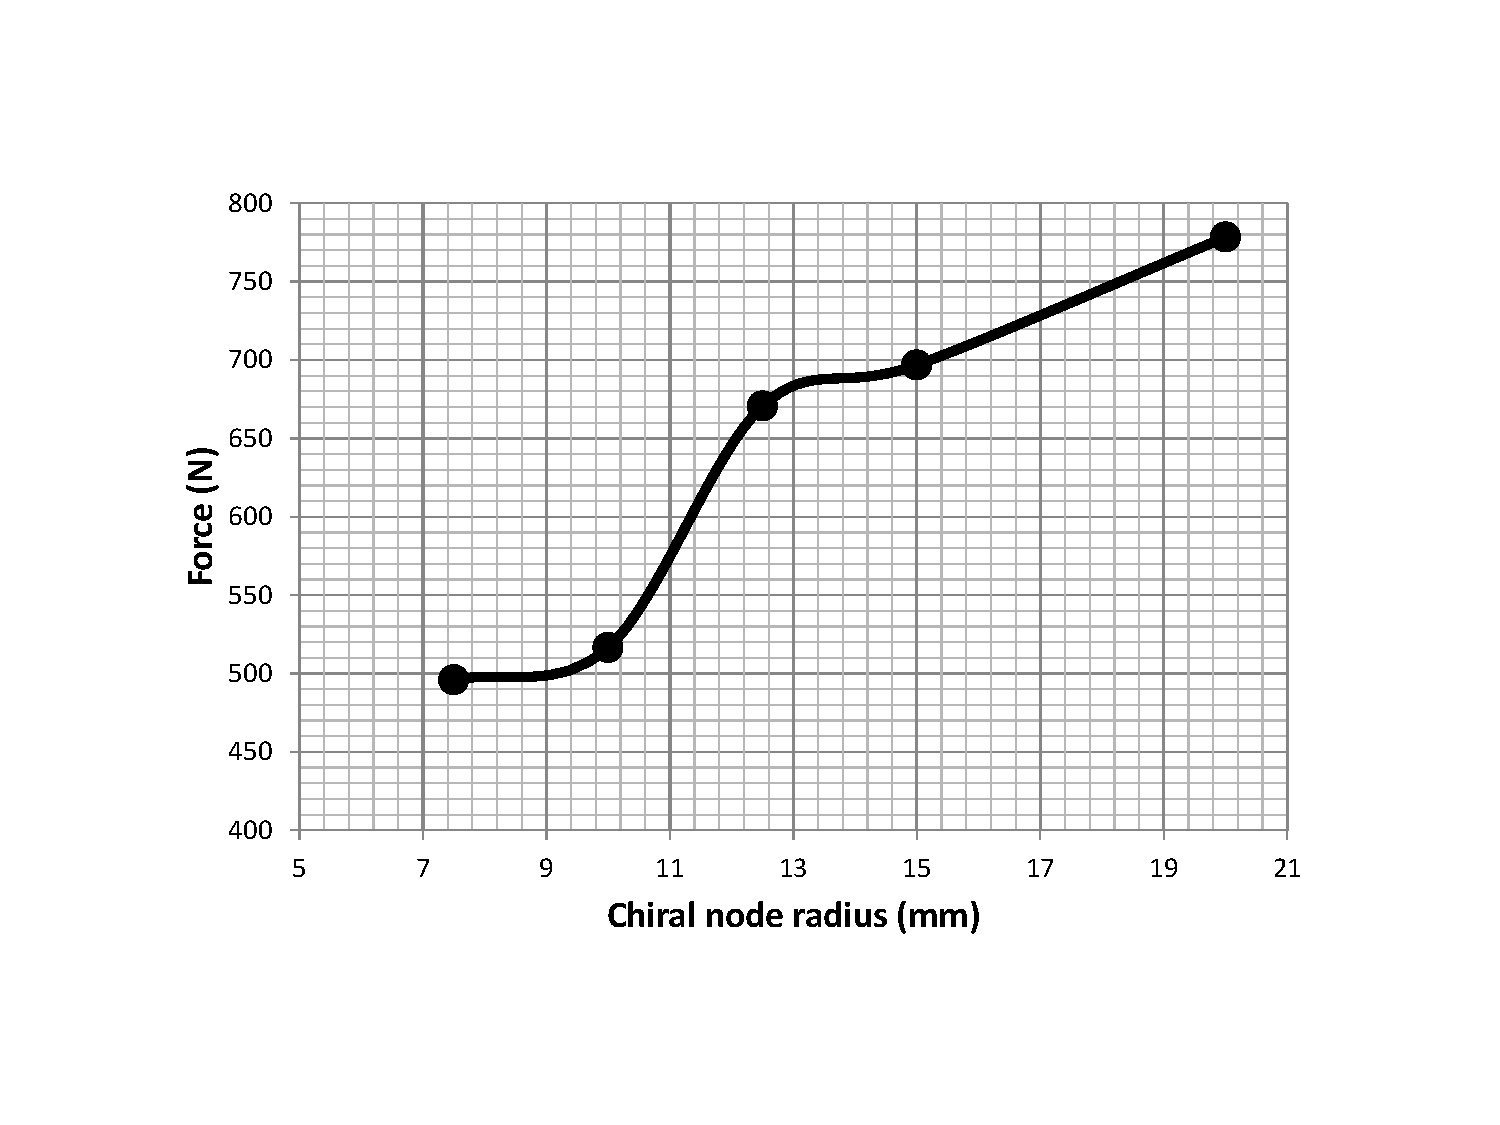
\includegraphics[width=0.8 \textwidth]{figures/result-sim/r/force_r}
        \caption[Force that induces the structure to collapse as a function of the chiral node depth]{Force that induces the structure to collapse as a function of the chiral node radius \chir.}\label{fig:force_r}
      \end{figure}

    \clearpage
    \subsubsection{Chiral ligament half length $L_{\mathrm{chi}}$}
      %
      %

      The numeric results obtained for the parametric study on the chiral ligament half length \chiL\ are shown in Table \ref{tab:para_L}. The geometrical meaning of this parameter can be seen in the sketch shown in Figure \ref{fig:lattice-internalParameters}. The displacement-force curve for the set of values analysed is shown in Figure \ref{fig:forceDisplacement-far-L}. This plot shows that the bigger the ligament half length is, the earlier the structure collapses after severe buckling of the ligaments at the root. For the case of \chiL$= 30$, the structure does not collapse because the higher ligaments length has incremented the buckling load.

      Again, in a further step, the force that causes the structure to collapse for a given value of the half length \chiL parameter is investigated. The resulting plot is shown in Figure \ref{fig:force_L}.

      \begin{table}[!htpb] %Results of L
        \centering
        \begin{tabular}{|l|l|l|l|l|l|l|l|l|}
        \hline
        \chiL & $\phi_{\mathrm{tip}}$ (deg) & $e(\phi_{\mathrm{tip}}) (\%)$ & $\tilde{\phi}_{\mathrm{tip}}$ (deg) & $e(\tilde{\phi}_{\mathrm{tip}}) (\%)$ & $v_{\mathrm{max}}$ & $\hat{z}_{v_{\mathrm{max}}}$ & $\hat{x}_{v_{\mathrm{max}}}$ \\ \hline
        30 & -0.181 & 13.106 & -0.131 & -8.951  & -1.101  & 1 & 0.602 \\ \hline
        50 & -1.596 & 14.222 & -0.203 & -18.444 & -14.267 & 1 & 0.334 \\ \hline
        70 & -3.252 & 13.574 & -0.204 & -8.297  & -24.022 & 1 & 0.463 \\ \hline
        \end{tabular}
        \caption[Results from the parametric study on chiral ligament half length]{Results from the parametric study on chiral ligament half length \chir. The results show the mean twist at the tip of the wing-box for the Abaqus nonlinear simulation $\phi_{\mathrm{tip}}$ and for the linear simulation $\tilde{\phi}_{\mathrm{tip}}$. The maximum relative error of the mean calculation, expressed as percentage, for these two magnitudes is $e(\phi_{\mathrm{tip}})$ and $e(\tilde{\phi}_{\mathrm{tip}})$, respectively. The table also shows the maximum vertical displacement $v_{\mathrm{max}}$ among all the mesh nodes located on the upper skin of the wing-box and the dimensionless position in the spanwise direction $\hat{x}_{v_{\mathrm{max}}}$ and in the chordwise direction $\hat{z}_{v_{\mathrm{max}}}$ of the node that shows $v = v_{\mathrm{max}}$.}
        \label{tab:para_L}
      \end{table}

      \begin{figure}[!htpb] %force_displacement-far
        \centering
        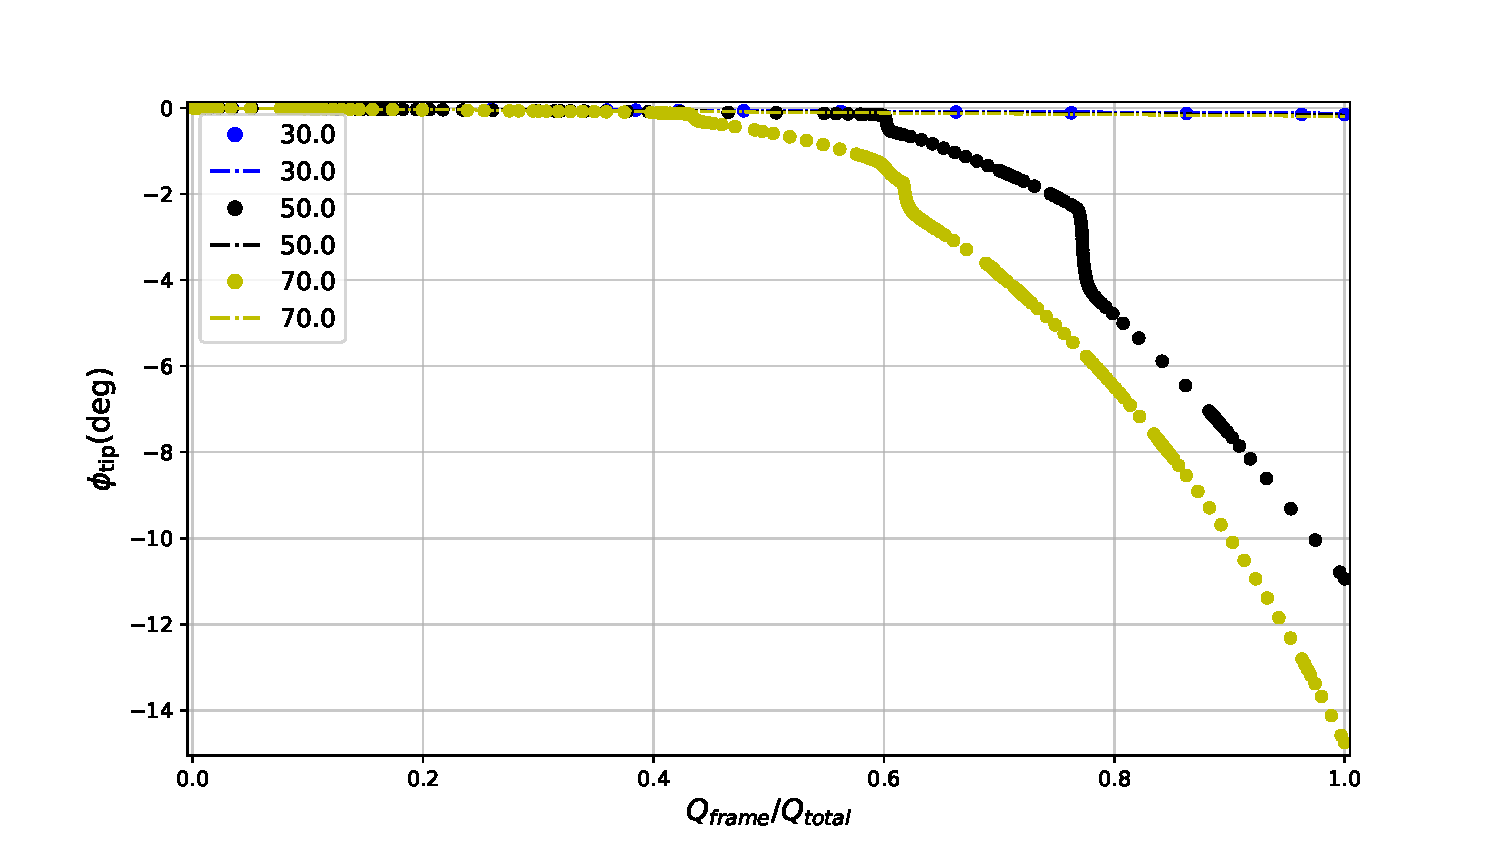
\includegraphics[width=0.8 \textwidth]{figures/result-sim/L/force_displacement-far}
        \caption[Displacement-force curve for various values of the chiral ligament half length]{Displacement-force curve for various values of the chiral ligament half length \chiL. The bigger the ligament half length is, the earlier that the structure will collapse after severe buckling of the ligaments at the root.}\label{fig:forceDisplacement-far-L}
      \end{figure}

      \begin{figure}[!htpb] %force_plot
        \centering
        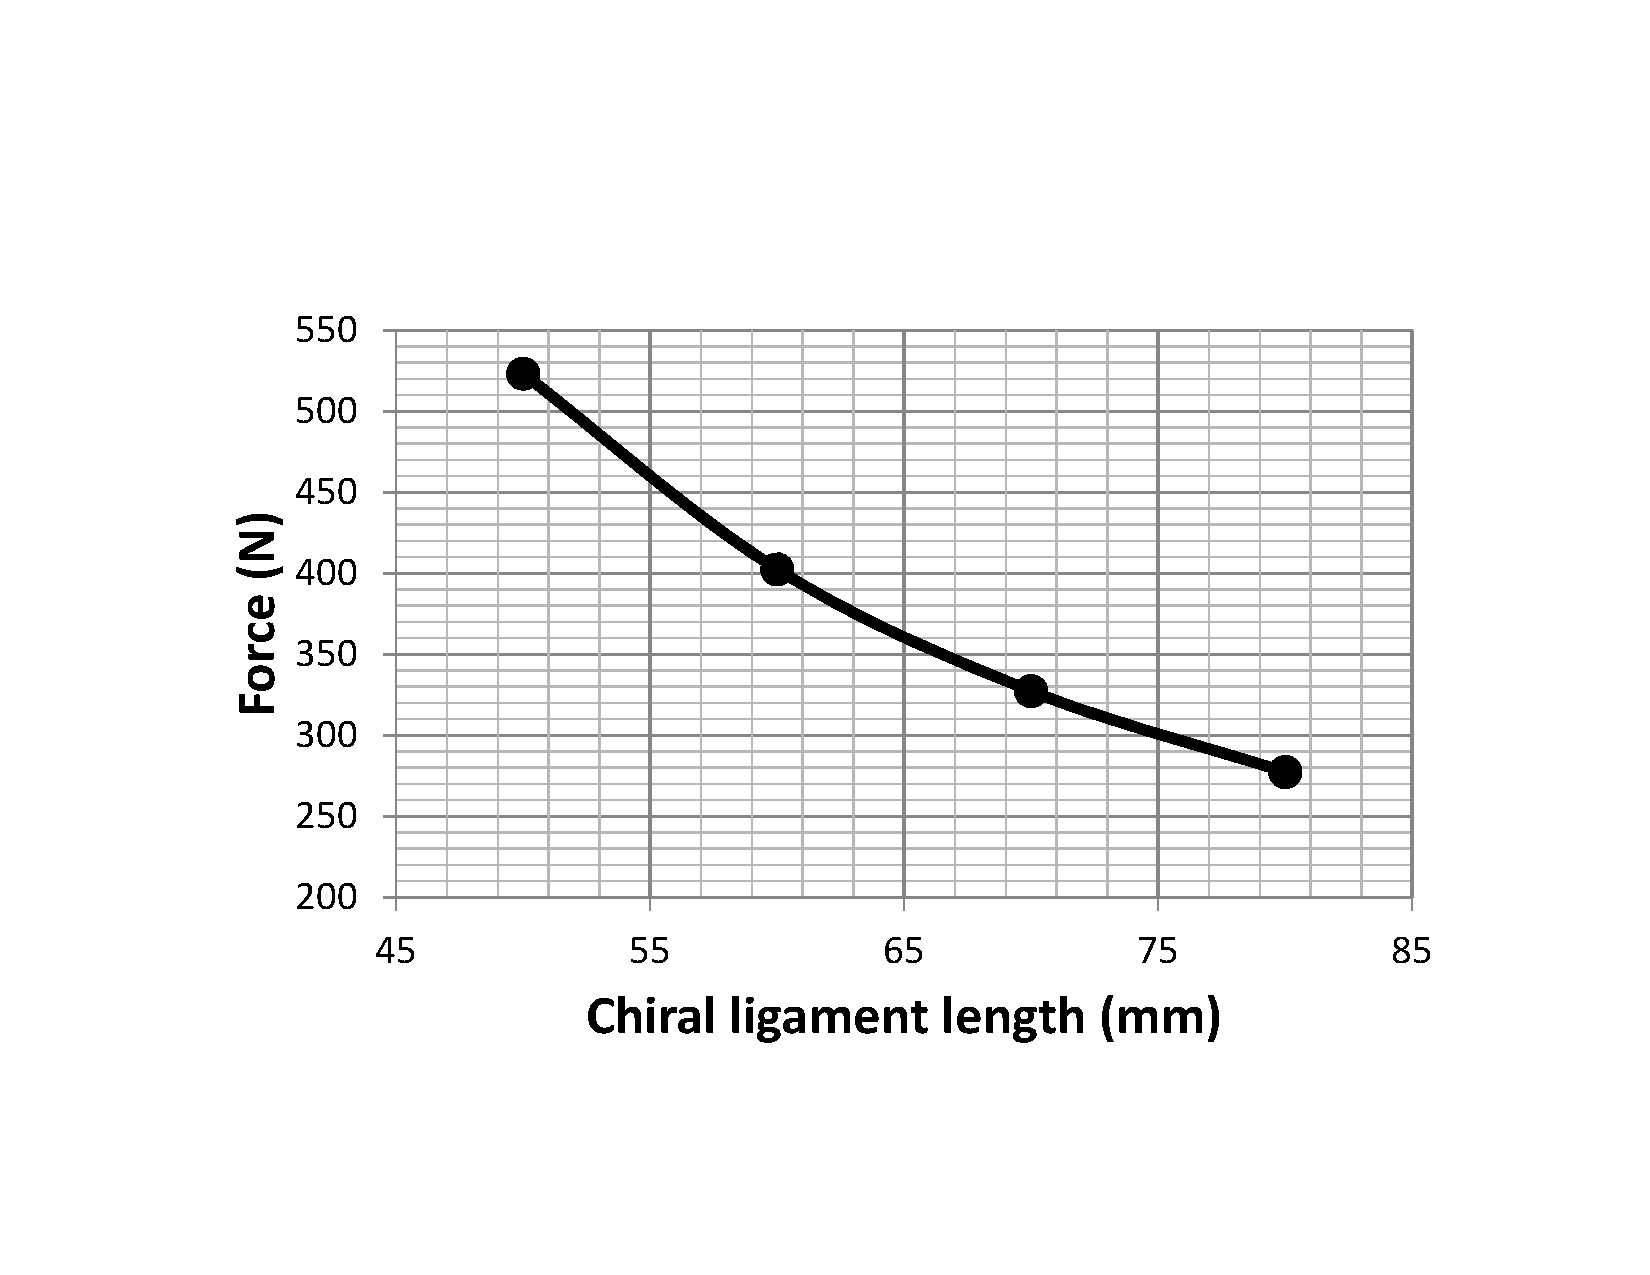
\includegraphics[width=0.8 \textwidth]{figures/result-sim/L/force_L}
        \caption[Force that induces the structure to collapse as a function of the chiral ligament half length]{Force that induces the structure to collapse as a function of the chiral ligament half length \chiL.}\label{fig:force_L}
      \end{figure}

    \clearpage
    \subsubsection{Chiral structure thickness $t_{\mathrm{chi}}$}
      %

      The results for the parametric study performed on the chiral structure thickness \chit are shown in Table \ref{tab:para_chi_t}. This parameter represents the wall thickness assigned to all the shell elements that form the lattice structure part, shown in Figure \ref{fig:lattice-internalParameters}. The displacement-force curve is shown in Figure \ref{fig:forceDisplacement-far-chiral-t}. Here it can be seen that a thicker chiral structure delays the structure collapse. An interesting aspect to be considered is that the more bigger the thickness \chit is, the bigger the magnitude of the sudden wing-box twist adaptation is.

      Finally, the required force to induce the structure collapse is plot against the corresponding value of the chiral structure thickness \chit, resulting on the curve shown in Figure \ref{fig:force_chiral_t}.

      \begin{table}[!htpb] %Results of chiral thickness
        \centering
        \begin{tabular}{|l|l|l|l|l|l|l|l|l|}
        \hline
        \chit & $\phi_{\mathrm{tip}}$ (deg) & $e(\phi_{\mathrm{tip}}) (\%)$ & $\tilde{\phi}_{\mathrm{tip}}$ (deg) & $e(\tilde{\phi}_{\mathrm{tip}}) (\%)$ & $v_{\mathrm{max}}$ & $\hat{z}_{v_{\mathrm{max}}}$ & $\hat{x}_{v_{\mathrm{max}}}$ \\ \hline
        0.2 & -1.413 & 11.363 & -0.233 & -15.24  & -10.646 & 1 & 0.546 \\ \hline
        0.4 & -1.331 & 11.406 & -0.206 & -15.187 & -12.654 & 1 & 0.334 \\ \hline
        0.6 & -0.699 & 14.276 & -0.193 & -18.502 & -7.311  & 1 & 0.546 \\ \hline
        0.8 & -0.186 & 6.856  & -0.125 & -12.046 & -2.039  & 1 & 0.546 \\ \hline
        \end{tabular}
        \caption[Results from the parametric study on chiral structure thickness]{Results from the parametric study on chiral structure thickness \chit. The results show the mean twist at the tip of the wing-box for the Abaqus nonlinear simulation $\phi_{\mathrm{tip}}$ and for the linear simulation $\tilde{\phi}_{\mathrm{tip}}$. The maximum relative error of the mean calculation, expressed as percentage, for these two magnitudes is $e(\phi_{\mathrm{tip}})$ and $e(\tilde{\phi}_{\mathrm{tip}})$, respectively. The table also shows the maximum vertical displacement $v_{\mathrm{max}}$ among all the mesh nodes located on the upper skin of the wing-box and the dimensionless position in the spanwise direction $\hat{x}_{v_{\mathrm{max}}}$ and in the chordwise direction $\hat{z}_{v_{\mathrm{max}}}$ of the node that shows $v = v_{\mathrm{max}}$.}
        \label{tab:para_chi_t}
      \end{table}

      \begin{figure}[!htpb] %force_displacement-far
        \centering
        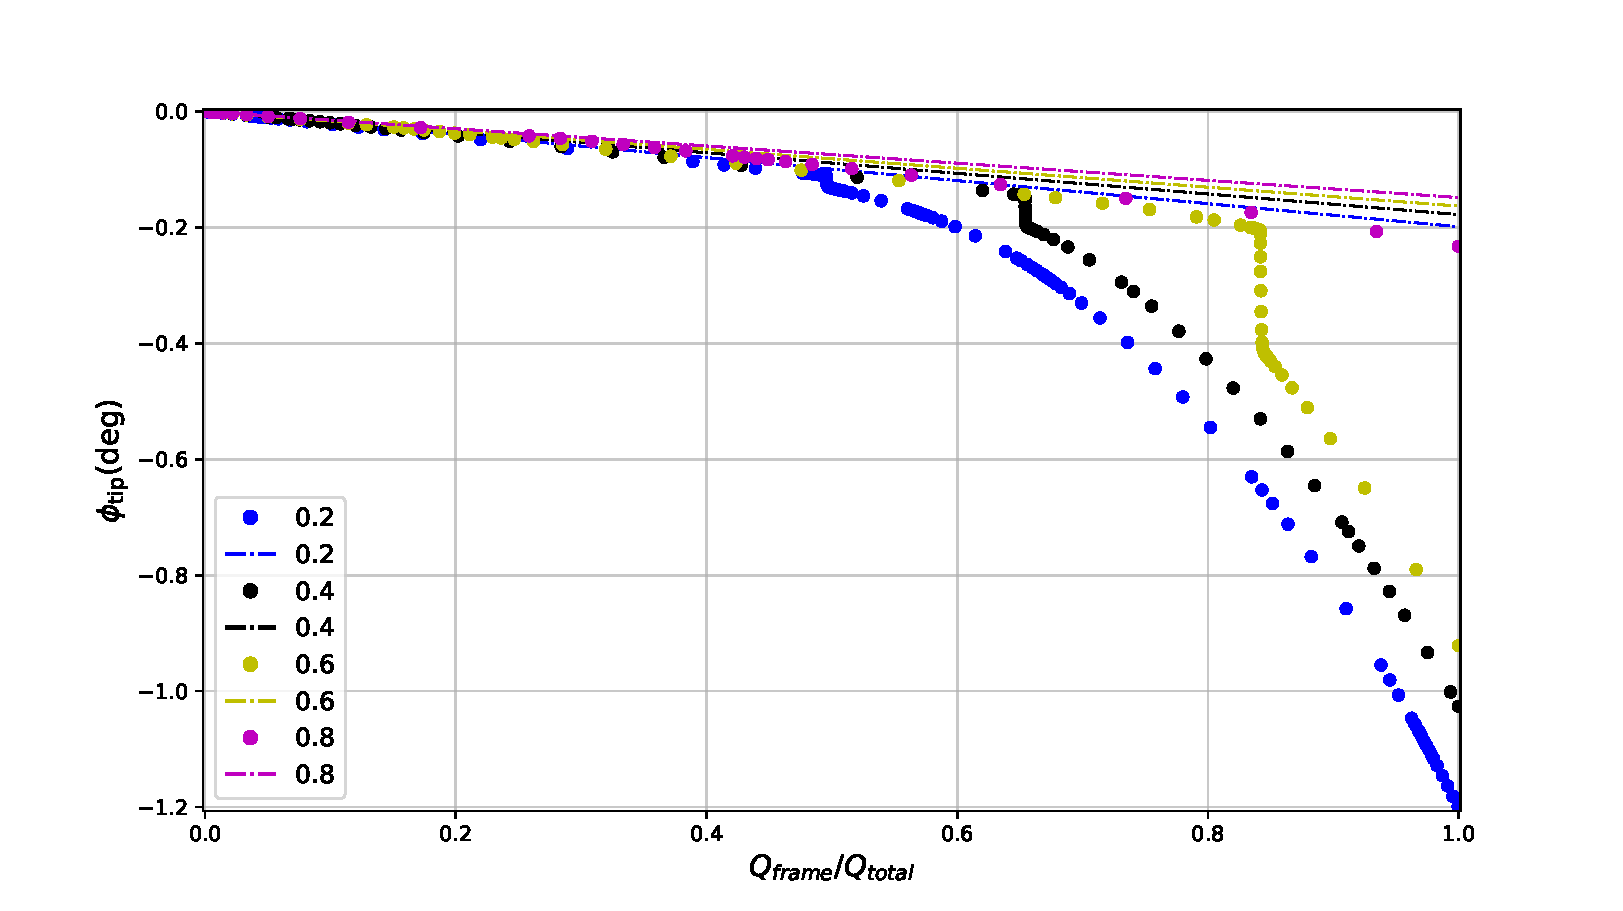
\includegraphics[width=0.8 \textwidth]{figures/result-sim/chiral_t/force_displacement-far}
        \caption[Displacement-force curve for various values of the chiral structure thickness]{Displacement-force curve for various values of the chiral structure thickness \chit. The bigger the ligament half length is, the earlier that the structure will collapse after severe buckling of the ligaments at the root.}\label{fig:forceDisplacement-far-chiral-t}
      \end{figure}

      \begin{figure}[!htpb] %force_plot
        \centering
        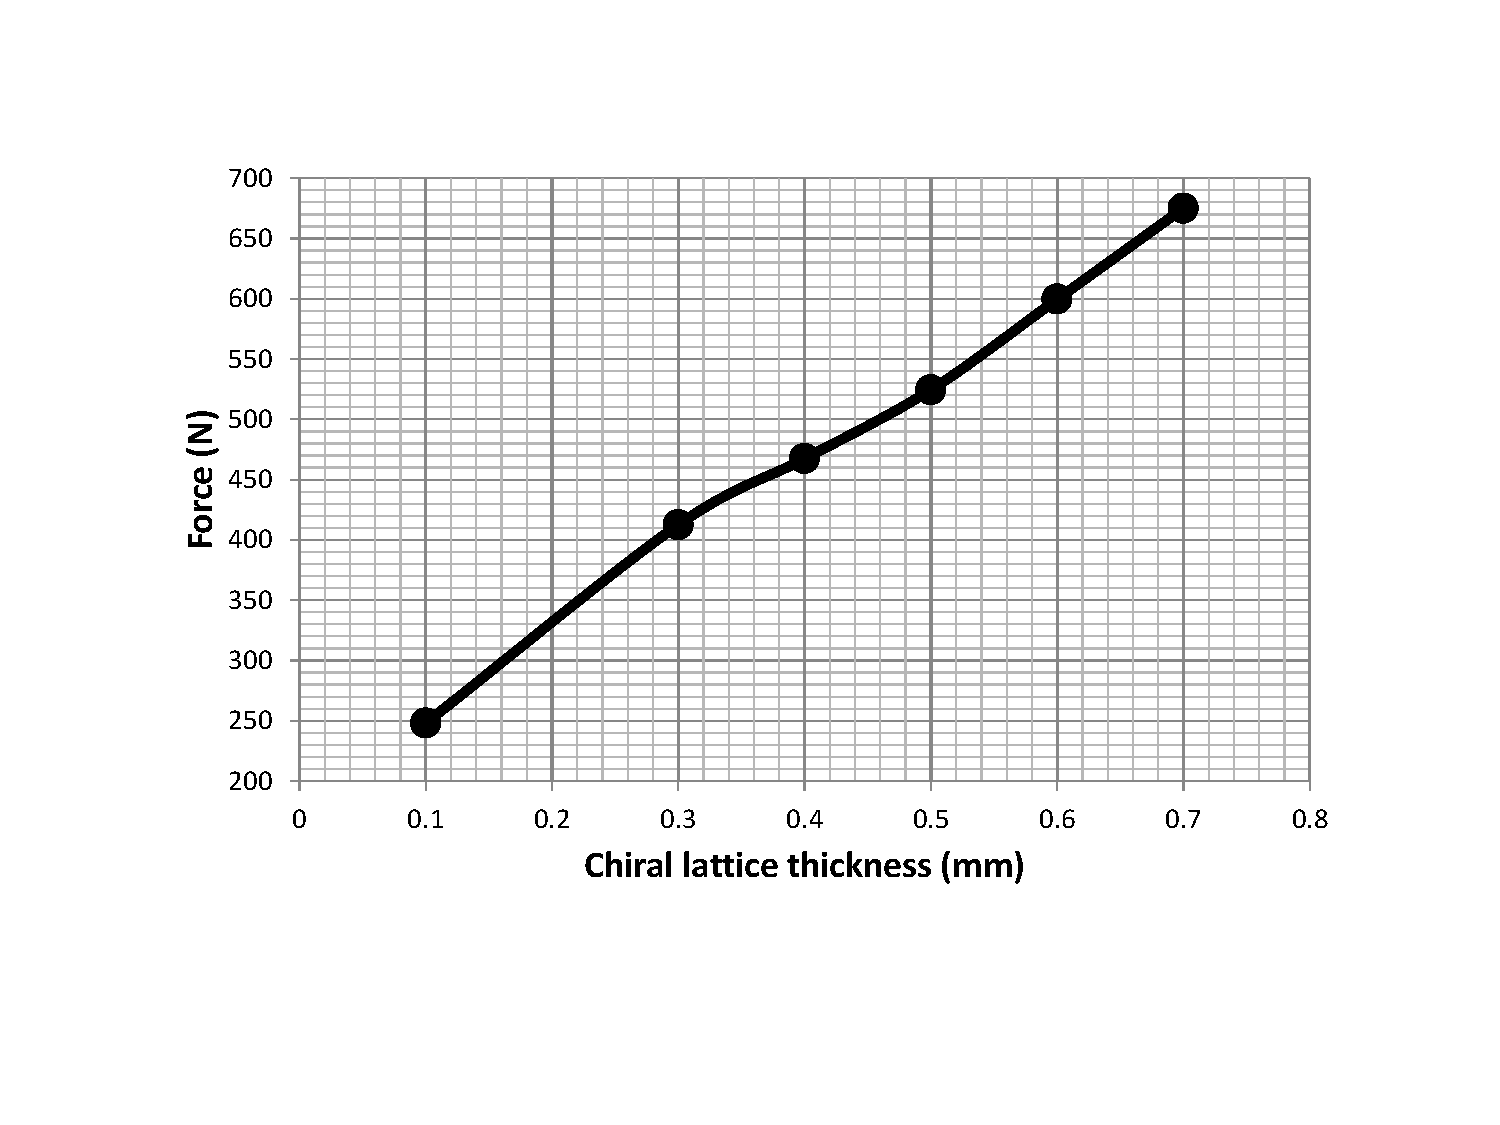
\includegraphics[width=0.8 \textwidth]{figures/result-sim/chiral_t/force_chiral_t}
        \caption[Force that induces the structure to collapse as a function of the chiral structure thickness]{Force that induces the structure to collapse as a function of the chiral structure thickness \chit.}\label{fig:force_chiral_t}
      \end{figure} 